% !TeX encoding = UTF-8
% !TeX program = xelatex
% !TeX spellcheck = en_US

\documentclass[degree=master, main-language=english, language=english]{thuthesis}
  % 学位 degree:
  %   doctor | master | bachelor | postdoc
  % 学位类型 degree-type:
  %   academic(默认)| professional


% 论文基本配置,加载宏包等全局配置
% !TeX root = ./thuthesis-example.tex

% 论文基本信息配置

\thusetup{
  %******************************
  % 注意:
  %   1. 配置里面不要出现空行
  %   2. 不需要的配置信息可以删除
  %   3. 建议先阅读文档中所有关于选项的说明
  %******************************
  %
  % 输出格式
  %   选择打印版(print)或用于提交的电子版(electronic),前者会插入空白页以便直接双面打印
  %
  output = print,
  %
  % 标题
  %   可使用“\\”命令手动控制换行
  %
  title  = {针对于物联网环境研究之下的真实-虚拟世界连接界面},
  title* = {Real-virtual world connection interface for research in IoT environment},
  %
  % 学位
  %   1. 学术型
  %      - 中文
  %        需注明所属的学科门类,例如:
  %        哲学、经济学、法学、教育学、文学、历史学、理学、工学、农学、医学、
  %        军事学、管理学、艺术学
  %      - 英文
  %        博士:Doctor of Philosophy
  %        硕士:
  %          哲学、文学、历史学、法学、教育学、艺术学门类,公共管理学科
  %          填写“Master of Arts“,其它填写“Master of Science”
  %   2. 专业型
  %      直接填写专业学位的名称,例如:
  %      教育博士、工程硕士等
  %      Doctor of Education, Master of Engineering
  %   3. 本科生不需要填写
  %
  degree-name  = {工学硕士},
  degree-name* = {Master of Science},
  %
  % 培养单位
  %   填写所属院系的全名
  %
  department = {计算机科学与技术系},
  %
  % 学科
  %   1. 学术型学位
  %      获得一级学科授权的学科填写一级学科名称,其他填写二级学科名称
  %   2. 工程硕士
  %      工程领域名称
  %   3. 其他专业型学位
  %      不填写此项
  %   4. 本科生填写专业名称,第二学位论文需标注“(第二学位)”
  %
  discipline  = {计算机科学与技术},
  discipline* = {Computer Science and Technology},
  %
  % 姓名
  %
  author  = {费杰},
  author* = {Ivachev Fedor},
  %
  % 指导教师
  %   中文姓名和职称之间以英文逗号“,”分开,下同
  %
  supervisor  = {喻纯, 副研究员},
  supervisor* = {Associate Professor Yu Chun},
  %
  % 副指导教师
  %
 % associate-supervisor  = {陈文光, 教授},
  %associate-supervisor* = {Professor Chen Wenguang},
  %
  % 联合指导教师
  %
  % joint-supervisor  = {某某某, 教授},
  % joint-supervisor* = {Professor Mou Moumou},
  %
  % 日期
  %   使用 ISO 格式;默认为当前时间
  %
  % date = {2019-07-07},
  %
  % 是否在中文封面后的空白页生成书脊(默认 false)
  %
  include-spine = false,
  %
  % 密级和年限
  %   秘密, 机密, 绝密
  %
  % secret-level = {秘密},
  % secret-year  = {10},
  %
  % 博士后专有部分
  %
  % clc                = {分类号},
  % udc                = {UDC},
  % id                 = {编号},
  % discipline-level-1 = {计算机科学与技术},  % 流动站(一级学科)名称
  % discipline-level-2 = {系统结构},          % 专业(二级学科)名称
  % start-date         = {2011-07-01},        % 研究工作起始时间
}

% 载入所需的宏包

% 可以使用 nomencl 生成符号和缩略语说明
% \usepackage{nomencl}
% \makenomenclature

% 表格加脚注
\usepackage{threeparttable}

% 表格中支持跨行
\usepackage{multirow}

% 固定宽度的表格。放在 hyperref 之前的话,tabularx 里的 footnote 显示不出来。
% \usepackage{tabularx}

% 跨页表格
% \usepackage{longtable}

\usepackage{float}
\usepackage{placeins}
\usepackage[dvips]{hyperref}

% 量和单位
\usepackage{siunitx}

% 定理类环境宏包
\usepackage{amsthm}
% 也可以使用 ntheorem
% \usepackage[amsmath,thmmarks,hyperref]{ntheorem}

% 参考文献使用 BibTeX + natbib 宏包
% 顺序编码制
\usepackage[sort]{natbib}
\bibliographystyle{thuthesis-numeric}

% 著者-出版年制
% \usepackage{natbib}
% \bibliographystyle{thuthesis-author-year}

% 本科生参考文献的著录格式
% \usepackage[sort]{natbib}
% \bibliographystyle{thuthesis-bachelor}

% 参考文献使用 BibLaTeX 宏包
% \usepackage[backend=biber,style=thuthesis-numeric]{biblatex}
% \usepackage[backend=biber,style=thuthesis-author-year]{biblatex}
% \usepackage[backend=biber,style=apa]{biblatex}
% \usepackage[backend=biber,style=mla-new]{biblatex}
% 声明 BibLaTeX 的数据库
% \addbibresource{ref/refs.bib}

% 定义所有的图片文件在 figures 子目录下
\graphicspath{{figures/}}

% 数学命令
\newcommand\dif{\mathop{}\!\mathrm{d}}  % 微分符号

% hyperref 宏包在最后调用
\usepackage{hyperref}
\usepackage{mathtools}




\begin{document}

% 封面
\maketitle


% 学位论文指导小组、公开评阅人和答辩委员会名单
% !TeX root = ../thuthesis-example.tex

\begin{committee}[name={学位论文指导小组、公开评阅人和答辩委员会名单}]

  \newcolumntype{C}[1]{@{}>{\centering\arraybackslash}p{#1}}

%   \section*{指导小组名单}

%   \begin{center}
%     \begin{tabular}{C{3cm}C{3cm}C{9cm}@{}}
%       李XX & 教授     & 清华大学 \\
%       王XX & 副教授   & 清华大学 \\
%       张XX & 助理教授 & 清华大学 \\
%     \end{tabular}
%   \end{center}


  \section*{公开评阅人名单}

  \begin{center}
    \begin{tabular}{C{3cm}C{3cm}C{9cm}@{}}
      陶霖密 & 副研究员   & 清华大学                    \\
      胡晓林 & 副教授  & 清华大学                  %  \\
    %   邓志东 & 教授 & 清华大学 \\
    \end{tabular}
  \end{center}


  \section*{答辩委员会名单}

  \begin{center}
    \begin{tabular}{C{2.75cm}C{2.98cm}C{4.63cm}C{4.63cm}@{}}
      主席 & 朱军                  & 教授                    & 清华大学       \\
      委员 &胡晓林                  & 副教授                    & 清华大学       \\
          & 陶霖密 & 副研究员 & 清华大学 \\
          & 孙茂松                  & 教授                    & 清华大学       \\
          & 喻纯                 & 副研究员                  & 清华大学       \\
          & 唐杰                 & 教授                  & 清华大学       \\
      秘书 & 戴音                  & 讲师              & 清华大学       \\
    \end{tabular}
  \end{center}

\end{committee}



% 也可以导入 Word 版转的 PDF 文件
% \begin{committee}[file=figures/committee.pdf]
% \end{committee}


% 使用授权的说明
\copyrightpage
% 将签字扫描后授权文件 scan-copyright.pdf 替换原始页面
% \copyrightpage[file=scan-copyright.pdf]

\frontmatter
% !TeX root = ../thuthesis-example.tex

% 中英文摘要和关键字

\begin{abstract}

近年来,泛在感知、人机交互等计算机技术不断发展,使得万物互联、智能空间逐渐成为可能:在服饰、家具等物品中嵌入系统级芯片或微控制器,可实现传感器数据的获取和储存,对其进行分析并共享到互联网,并通过嵌入式麦克风,扬声器和信息显示器等输入输出接口与用户进行信息交互。随5G 和 6G 网络的快速发展,我们可以期待未来对成千上万台设备的连接可以做到快速且节能。设备之间更高数据的共享以及对大数据分析的改进提升,促进着物联网的进一步发展。而对于智能空间的研发来说,目前由于缺乏能够使物理设备快速集成到现实世界应用场景的标准软件,广大应用开发者在针对个例应用进行定制开发,产生大量重复的工程实现,导致严重的人力和资源的浪费。同时,随交互场景智能化不断提高,场景复杂性也不断提升,因而导致交互场景的开发成本高周期长;交互验证需要依托场景完成,验证滞后导致交互效果难以保证符合预期,进而需要更多轮次更长周期的修正迭代。

同时,虚拟现实技术近来得到了飞速地发展,并且伴随着手部识别技术以及虚拟现实头戴显示器设备的革新,已不仅仅可用于娱乐应用,而且还得以应用于医疗保健,教育,和科学研究。

作者在此提出了一种同步机制,该机制可以根据虚拟世界中的动作和事件一致同步更新真实和虚拟设备状态,反之亦然——将应用于真实设备中的动作同步到虚拟世界中去。本文所探讨的问题为,是否可以借助虚拟现实交互设备来开发这种机制,并将其用于研发创新智能空间和交互设备。本论文的主要贡献在于:
  
\begin{enumerate}
    \item 创新提出了虚实融合AIoT开发和测试平台,用于开发物联网设备、场景和交互方法,可显著节省开发成本,提高效率。
    \item 提出虚实设备之间的数据同步机制,实现虚拟设备和物理设备的实时状态绑定,并支持设备之间互操作。
    \item 提供了NUIX Studio 开发工具包,具备丰富的可重用部件和功能,供研究人员快速开发AIoT 原型交互系统。
\end{enumerate}


  % 关键词用“英文逗号”分隔,输出时会自动处理为正确的分隔符
  \thusetup{
    keywords = {物联网, 虚拟现实, 人机交互},
  }
\end{abstract}

\begin{abstract*}

  In recent years processing power has become so cheap that making objects around us intelligent is no longer a challenge: using energy-efficient System-on-Chips or microcontrollers in clothes, furniture, toys, and other things helps to monitor our activity, store sensors' data, analyze it and share it to the Internet. Such smart things can interact with us using embedded microphones, speakers and information displays. The rapid development of 5G- and 6G-networks in the near future will make it possible to provide a fast and energy-efficient way to connect thousands of devices no longer attached to a single location. Higher data sharing between the devices and improved Big Data analysis will lead to further evolution of the Internet of Things. Developing new types of devices is an issue, since there is no standard software for their rapid integration into existing real-world scenarios.
   
  In the meantime, Virtual Reality has recently seen rapid development, and with the newer technique of hands recognition, as well as the evolution of Virtual Reality Headsets, it has proven itself as a great instrument not only for gaming purposes but for healthcare, education, and science.
   
  The author proposes a synchronization mechanism that keeps real and virtual devices up-to-date, according to actions and events in the virtual world and applying actions from the real devices to the virtual world. This thesis asks if, with the help of Virtual Reality interaction devices, such a mechanism can be developed and used as a part of an instrument for research on new devices. The main contributions of this thesis include:
  
  \begin{enumerate}
      \item A novel hybrid virtuality-reality model for developing IoT devices and scenarios, which can significantly save development cost and improve efficiency. 
      \item A synchronization mechanism that binds the status of virtual devices and physical devices in real time, and supports inter-operations. 
      \item A development kit, called NUIX-Studio, for researchers to fast prototype AIoT projects, with a rich set of reusable widgets and functionalities. The spatial and temporal synchronization is used to keep the sensor states equal in real and virtual worlds.
  \end{enumerate}
  
  % Use comma as seperator when inputting
  \thusetup{
    keywords* = {IoT, VR, HCI},
  }
\end{abstract*}


% 目录
\tableofcontents


% 插图和附表清单
% \listoffiguresandtables  % 插图和附表清单
\listoffigures           % 插图清单
\listoftables            % 附表清单

% 符号对照表
% !TeX root = ../thuthesis-example.tex

\begin{denotation}[3cm]
  \item[IoT] Internet of Things
  \item[AIoT] Artificial Intelligence of Things
  \item[VR] Virtual Reality
  \item[AR] Augmented Reality
  \item[MR] Mixed Reality
  \item[HCI] Human-computer interaction
  \item[DB] Database
  \item[HMD] Head-mounted display
  \item[IoV] Internet of Vehicle
  \item[SOA] Service-oriented architecture
  \item[API] Application Programming Interface
  \item[DTO] Data Transfer Object
  \item[App] Application
\end{denotation}



% 也可以使用 nomencl 宏包,需要在导言区
% \usepackage{nomencl}
% \makenomenclature

% 在这里输出符号说明
% \printnomenclature[3cm]

% 在正文中的任意为都可以标题
% \nomenclature{PI}{聚酰亚胺}
% \nomenclature{MPI}{聚酰亚胺模型化合物,N-苯基邻苯酰亚胺}
% \nomenclature{PBI}{聚苯并咪唑}
% \nomenclature{MPBI}{聚苯并咪唑模型化合物,N-苯基苯并咪唑}
% \nomenclature{PY}{聚吡咙}
% \nomenclature{PMDA-BDA}{均苯四酸二酐与联苯四胺合成的聚吡咙薄膜}
% \nomenclature{MPY}{聚吡咙模型化合物}
% \nomenclature{As-PPT}{聚苯基不对称三嗪}
% \nomenclature{MAsPPT}{聚苯基不对称三嗪单模型化合物,3,5,6-三苯基-1,2,4-三嗪}
% \nomenclature{DMAsPPT}{聚苯基不对称三嗪双模型化合物(水解实验模型化合物)}
% \nomenclature{S-PPT}{聚苯基对称三嗪}
% \nomenclature{MSPPT}{聚苯基对称三嗪模型化合物,2,4,6-三苯基-1,3,5-三嗪}
% \nomenclature{PPQ}{聚苯基喹噁啉}
% \nomenclature{MPPQ}{聚苯基喹噁啉模型化合物,3,4-二苯基苯并二嗪}
% \nomenclature{HMPI}{聚酰亚胺模型化合物的质子化产物}
% \nomenclature{HMPY}{聚吡咙模型化合物的质子化产物}
% \nomenclature{HMPBI}{聚苯并咪唑模型化合物的质子化产物}
% \nomenclature{HMAsPPT}{聚苯基不对称三嗪模型化合物的质子化产物}
% \nomenclature{HMSPPT}{聚苯基对称三嗪模型化合物的质子化产物}
% \nomenclature{HMPPQ}{聚苯基喹噁啉模型化合物的质子化产物}
% \nomenclature{PDT}{热分解温度}
% \nomenclature{HPLC}{高效液相色谱 (High Performance Liquid Chromatography)}
% \nomenclature{HPCE}{高效毛细管电泳色谱 (High Performance Capillary lectrophoresis)}
% \nomenclature{LC-MS}{液相色谱-质谱联用 (Liquid chromatography-Mass Spectrum)}
% \nomenclature{TIC}{总离子浓度 (Total Ion Content)}
% \nomenclature{\textit{ab initio}}{基于第一原理的量子化学计算方法,常称从头算法}
% \nomenclature{DFT}{密度泛函理论 (Density Functional Theory)}
% \nomenclature{$E_a$}{化学反应的活化能 (Activation Energy)}
% \nomenclature{ZPE}{零点振动能 (Zero Vibration Energy)}
% \nomenclature{PES}{势能面 (Potential Energy Surface)}
% \nomenclature{TS}{过渡态 (Transition State)}
% \nomenclature{TST}{过渡态理论 (Transition State Theory)}
% \nomenclature{$\increment G^\neq$}{活化自由能(Activation Free Energy)}
% \nomenclature{$\kappa$}{传输系数 (Transmission Coefficient)}
% \nomenclature{IRC}{内禀反应坐标 (Intrinsic Reaction Coordinates)}
% \nomenclature{$\nu_i$}{虚频 (Imaginary Frequency)}
% \nomenclature{ONIOM}{分层算法 (Our own N-layered Integrated molecular Orbital and molecular Mechanics)}
% \nomenclature{SCF}{自洽场 (Self-Consistent Field)}
% \nomenclature{SCRF}{自洽反应场 (Self-Consistent Reaction Field)}



% 正文部分
\mainmatter
% !TeX root = ../thuthesis-example.tex

\chapter{\MakeUppercase{Introduction}}

\section{Problem definition}

The Internet of Things (IoT) is expected to connect hundreds of billions of devices in less than a decade~\cite{simiscuka_synchronisation_2018}, with tens of billions of connected IoT devices already in existence around the world. This number is anticipated to keep increasing as Internet connectivity has become a standard feature for a significant number of electronic devices~\cite{hu_virtual_2021}. Many companies, such as Huawei, Baidu, Alibaba, Tencent, Google, Intel, etc., already have ways to integrate data coming from IoT devices~\cite{perera}. Although most of these products are restricted for use only with limited types or models of IoT devices, companies may come to standardize IoT devices in the next few years. Nowadays, most consumer IoT devices can be controlled by popular Smart assistants, such as Apple Siri, Amazon Alexa, Tencent Xiaowei, etc., or by SDKs, such as Apple HomeKit~\cite{perera}. Unified solutions make it possible to control all the devices using a phone, computer, or Smart Speaker.
On the other hand, controlling IoT devices by smartphones and Smart speakers does not provide the best user experience. The interaction techniques are limited: even though processing power per energy consumption has increased dramatically, and it is possible to have the processing power of high-performance PC of the 1990s in tiny devices such as smartwatches, there is no freedom of movement and data sharing. Even though 5G networks partly resolve this issue, for example by making it possible to create an Internet of Vehicle (IoV), the transmission bandwidth is still limited, causing severe safety consequences~\cite{hu_virtual_2021}. For example, when computations for interaction techniques such as hand gesture recognition cannot be performed on the IoT device due to its limited computing power, the sensing data must be transferred to a server, analyzed, and only then sent back to the sensing device to provide an output to the user.

The sixth-generation (6G) mobile network is expected to make possible new applications utilizing the increased speed and transmission of the network~\cite{huang_survey_2019, liao_information-centric_2021}. It is expected that a 6G network will be an improvement on the current 5G network and, therefore, provide faster data sharing between devices, which will in turn help overcome the issues stated in the previous paragraph. As soon as this becomes possible, the companies which adapt more quickly to the new standards will be more advanced on the IoT market. Development speed, in this case, is one of the most important factors for companies' success.

Nowadays, the standard ways of integrating newly-developed IoT devices inside the existing environment is to use virtual (or digital) twins or to build prototypes. In the first case, interaction with such devices takes place on a 2D interface, with a very rough simulation of user behavior, which leads to further underestimations of data analysis. In the second case, creating a prototype requires waiting for the IoT device's modeling, sending the schemes to the manufacturers, and then waiting for the prototype to be delivered. In both cases, the disadvantages lead to the possibility of losing market share, either because of lack of usability or because of being too late to enter a market already controlled by competitors. Companies and researchers need an instrument to avoid these disadvantages and integrate prototypes of devices inside the existing real-world IoT environment.

In this research, a solution for this issue is proposed: a platform for developing new IoT devices. The following section describes how using another prospective technology can help create the platform defined above.

\section{Research method}

The problem of defining an instrument for researching new types of IoT devices and integrating them in the existing real-world environments, which was introduced in the previous section, requires a solution. The solution must facilitate integration of real-world devices, and, second, interaction with virtual devices.

Like IoT, Virtual reality (VR), together with AR, is considered one of the essential application-level requirements of 6G. Both technologies can effectively utilize the increased speed and transmission of the sixth-generation network. The biggest companies, such as Facebook, invest billions in AR and VR research. Nearly 10000 employees, almost 20\% of the company staff, work on research in this field~\cite{sam_byford_almost_2021}. Research papers applying Virtual reality to almost every area, such as games, education, healthcare, or industry, can already be found. Companies selling Virtual Reality Headsets provide powerful APIs for integrating their devices inside different 3D engines \footnote{The Virtual reality market and 3D engine to be used in this research are discussed in the next chapter.}. Researchers can use these interfaces to create a platform for interacting with virtual IoT devices.

The idea of this research project is to integrate Virtual reality headsets into the IoT environment. In the 6G era, it will be possible to send large amounts of data with much smaller latency and much higher speed than that of 5G networks. Wi-Fi 6 (802.11ax standard) already provides acceptable high-quality streaming from VR headsets to the server, with minimal latency in local scenarios.

Nevertheless, only using Virtual reality headsets does not solve the issue defined in the previous section. The research task is to define a layer between a real-world IoT environment and the user as a researcher working to construct new IoT devices (Figure~\ref{fig:VR-IoTResearchPlatformLayer-figure}). The VR-IoT Research Platform is based on this layer. It enables users to perform research on IoT devices inside the IoT-VR environment.

\begin{figure} 
  \centering
  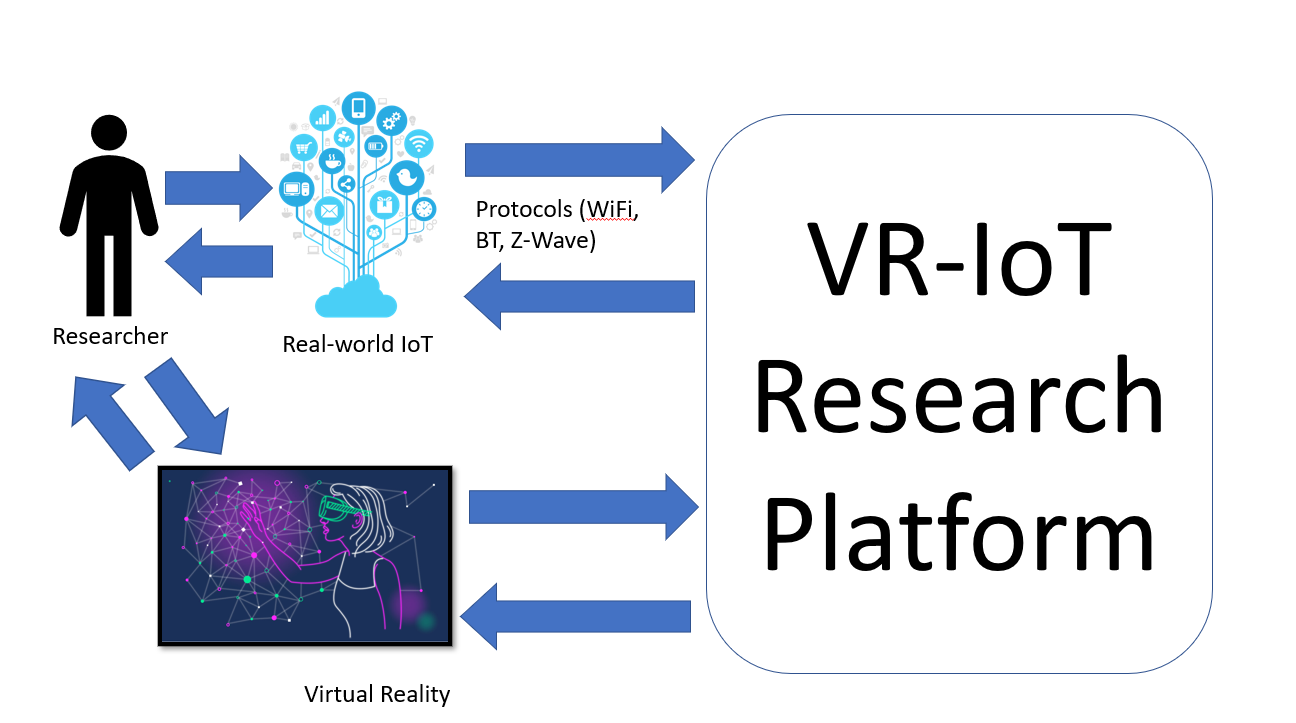
\includegraphics[width=0.9\linewidth]{figures/VR-IoTResearchPlatformLayer.png}
  \caption{VR-IoT Research Platform layer}
  \label{fig:VR-IoTResearchPlatformLayer-figure}
\end{figure}

The work is organized into seven Chapters. Chapter 2 reviews the literature on creating IoT devices using various methods, including VR. In Chapter 3, the author defines the platform architecture and gives its implementation details. In Chapter 4, the API for researchers to use the platform in the projects is introduced. Chapter 5 presents several tests that evaluate the platform performance on the network and in local scenarios. The platform usage examples are given in Chapter 6. Chapter 7 includes future directions for inquiry as well as the conclusion.


Summarizing the problem definition and research idea:

\begin{itemize}
    \item Problem definition: There is no instrument for quickly creating, testing, and integrating new IoT devices inside an existing real-world environment.  
    \item Research idea: Define a layer between real-world IoT devices and Virtual Reality. Create a prototype, evaluate its performance and usability, and summarize the outputs. Explain why the selected architecture can be used as the basis for a future product used to design new IoT devices.
\end{itemize}












% !TeX root = ../thuthesis-example.tex


\chapter{Literature review}

The literature review incorporates three sections: research on building an IoT platform without VR support, research on interacting with IoT devices in VR and AR, and lastly, research on creating an IoT-VR Platform.

\section{IoT device management}

Many companies already consider it profitable to use IoT in their businesses, but establishing connections between heterogeneous IoT devices is still a challenge. The existing frameworks that address this issue seem usually to be not user-friendly and not easy to use. 

The providers of IoT integration services for business state that their solutions can analyze large amounts of data from the connected IoT devices and then turn this data into actionable insights~\cite{software_ag_software_2020}. Businesses can then use the insights to lower energy consumption, analyze sensor data, etc.

Even if researchers can afford to pay a high price for data analysis, they still will not have access to the source code or to the data used for training the models. Users will need to pay for a subscription to the services. If users want to switch to another solution, it will require additional time and money.

In \cite{k_mohapatra_solution_2016} it is discussed how the framework for connecting heterogeneous devices should operate on incoming data. In this paper, the requirements for managing IoT are given: communication protocols, security and access control, and data analysis procedures. In section 4 of their paper, a Reference IoT-Architecture model is proposed. Each solution block, such as Data Lake or Event Broker, is briefly introduced, but neither implementation nor tests are provided.

The IoT Architectural Framework, proposed in~\cite{uviase_iot_2018}, is based on a Service Oriented Architecture (SOA). This paradigm is used to minimize system integration problems. But when the number of services increases, the solution's performance can drop. Minimum measures for easily integrating an IoT framework are proposed \footnote{These measures are used for building a VR-IoT platform prototype in chapter 3 of this paper.} The authors introduce several existing IoT frameworks based on the SOA paradigm, and propose their own approach. As stated in the paper, the framework has not been implemented.  Nevertheless, the authors believe that the proposed framework can help the IoT community to understand how to solve the integration problem.

Compared to \cite{k_mohapatra_solution_2016}, in \cite{ahmad_software_2021} authors provide a deeper explanation of how to create an Internet Of Things Driven Data Analytics by using an evidence-based software engineering approach. The authors have created a criteria-based framework by evaluating different activities for the 17 listed Internet of Things Driven Data Analytics applications. As a result, each of the applications was assigned to a specific domain, such as Disaster Management or Environmental Monitoring. Even though each of the listed criteria was fulfilled satisfactorily for at least one solution, none of the solutions could be considered universal. Still, they can be integrated into other solutions, as well as in the VR-IoT Research Platform.

In Chapter 1, we mentioned that building 6G could influence the IoT market. In \cite{guo_enabling_2021} a comprehensive study was done, explaining how the limitations on massive IoT 5G can be overcome using 6G networks. It was explained how machine learning and blockchain could play a primary role in IoT ecosystems. New technologies can be supported, such as holographic communications, which can be easily tested in the VR-IoT Research Platform.

\section{Interaction with IoT devices in VR and AR}

Augmented reality is used to overlay digital objects onto the objects surrounding us in real life. Extra virtual elements can be attached to real-world devices.

Rendering digital devices for Augmented reality and Virtual reality is different: in Augmented reality, it is impossible to replace the element placed in the real world with a virtual one. Creating a Virtual reality environment similar to the real-world environment requires more time and effort than scanning objects to use them in Augmented reality. But, as a result, researchers can have more freedom to make changes such as those to object parameters. 
In \cite{ankireddy_augmented_2019} authors developed an image processing-based approach to control a specific device in the real-world by pointing at it with their phone camera and pressing the button (turn the fan On and Off). Their solution is simple, but at the same time, it shows that it is possible to control IoT devices inside AR without using Mixed reality headsets, reducing the cost of development. Similar results were achieved in \cite{jo_-situ_2016}, where a generic AR framework for managing IoT devices was proposed, and in \cite{alam_augmented_2017} for creating a safety system by viewing monitoring information on an AR device screen when pointing at the object.

One of the most popular Mixed reality headsets is Microsoft Hololens. The device developers provide an API for hand tracking and spatial awareness~\cite{MRTK2021}. In \cite{sun_magichand_2019} the authors proposed a Deep learning approach to create a tool for interacting with IoT devices using hand gestures registered by a Hololens headset. 

Cities such as Shanghai, New York, Moscow can already be considered Smart cities because they have been implementing Smart solutions for several years~\cite{vershinina_smart_2016}. Using Augmented and Virtual reality can help in creating IoT solutions for such Smart cities and networks, as reported in ~\cite{chakareski_uav-iot_2019, carneiro_bim_2018}. As for other domains, in \cite{paul_role_2019} it was shown that AR and VR, combined with IoT, could be used for Smart education, and in \cite{jang_building_2019-1}, for energy management. In sum, using AR and VR for managing IoT has proven to be effective.

\section{IoT-VR platforms}

The current research would have had no novelty if a method for creating new IoT devices inside VR already existed. Fortunately, none of the following articles is focused on providing such a platform. Nonetheless, they are still helpful for considering VR-IoT platform development.

The next-generation network will influence the IoT market, as stated previously. In \cite{liao_information-centric_2021}, the authors provide their solution for integrating AR/VR inside a 6G massive IoT environment.

As mentioned in the previous section, using VR for IoT research requires building a virtual environment. Nowadays, most VR headsets provide 6 degrees of freedom, which means that it is possible to simultaneously move in the real world and in the virtual world. In \cite{you_internet_2018} the authors research how IoT can be used to create seamless virtual reality space with 360-degree photos and videos.

In \cite{myeong-in_choi_design_2017, simiscuka_synchronisation_2018, simiscuka_real-virtual_2019, krishnan_performance_2020} VR-IoT platforms were proposed, but none of the articles focused on implementing a universal solution that can be used for developing new devices in the VR-IoT environment. Instead, only demos for particular devices were implemented.

Finally, in \cite{hu_virtual_2021} the authors provided research on the VR headsets market and introduced several VR-IoT environment applications. The authors mainly focused on VR streaming solutions.

Overall, various examples of using VR for IoT were proposed in the literature. The collected information can be summarized into the following insights:
\begin{enumerate}
    \item Today's IoT market is diverse. There are applications for most of the domains of Smart environments, but no universal solution exists;
   \item The SOA paradigm can be applied to create an IoT platform that minimizes integration problems;
    \item 6G networks will enable using new types of IoT devices based on Deep Learning and blockchain. The increased network speed will allow more advanced IoT interaction and Data Analysis;
    \item AR can enrich operation with real-world IoT devices by layering extra data on top of them. Detection of the IoT devices in AR can be performed using smartphone cameras to lower costs;
    \item Synchronization between real IoT devices and their virtual copies is possible with relatively low latency for a local-based approach.
\end{enumerate}

In the next Chapter, the VR-IoT Platform design and implementation details are provided.
% !TeX root = ../thuthesis-example.tex

\chapter{VR-IoT Research Platform}

% !TeX root = ../thuthesis-example.tex

\chapter{\MakeUppercase{NUIX-Studio Development kit}}

NUIX-Studio Development Kit helps researchers to fast prototype AIoT projects. This chapter briefly introduces each of its components, which are listed below:
\begin{enumerate}
    \item Things designer;
    \item Complex computations API;
    \item API and tools for IoT data visualization and analysis;
    \item API for creating Widgets.
\end{enumerate}

\section{Things Designer}

By using a block structure to represent devices, researchers can modify various parameters of existing devices by changing specific blocks and can create new devices by combining the blocks. This action is possible in a tool called Things designer. This tool is described in detail below.

The Semantic model is visualized inside the Web interface. Researchers can assign Widgets for each of the Items and group the Items together. After the setup is completed, researchers can further develop new devices inside the NUIX-Studio App. Next, they can create new Widgets in Virtual reality and connect them to the existing Items. The position for each of the Widgets is added to the Semantic model as an Item. Having set the Widget's position and other parameters, the user can exit the application on a device and then continue research using a different device or analyze the Item data stored on the server. 

There is a variety of different Widgets available for users. For example, a door open/close sensor with a light indicator can be combined of a Contact sensor Widget and Light Switch Widget (Figure~\ref{fig:PersistenceExample-figure}). Even though the Widgets are created virtually, they get added to the openHAB database. As already mentioned, each Widget is associated with an Item, and the Items together compose a Thing. Thus, a Thing is created, consisting of two Items: a Contact sensor and a light Switch indicator. Further, developers can link the corresponding Channels to each of the Items. For example, researchers can add a Binding for a real-world light bulb, and a Binding for a real-world sensor for opening and closing doors, discover the devices automatically and add them to the model. Next, in the device editing window, bind the Contact sensor and Light Switch sensor to the newly created Items. Thus, the light bulb will light up both in the real and virtual worlds when at least one of the doors is open. The developer can also set the initial state for the open door, solving the problem of synchronizing the door position in the real and virtual worlds. 

\begin{figure}
  \centering
  \subcaptionbox{Opened door.\label{fig:dooropen}}
    {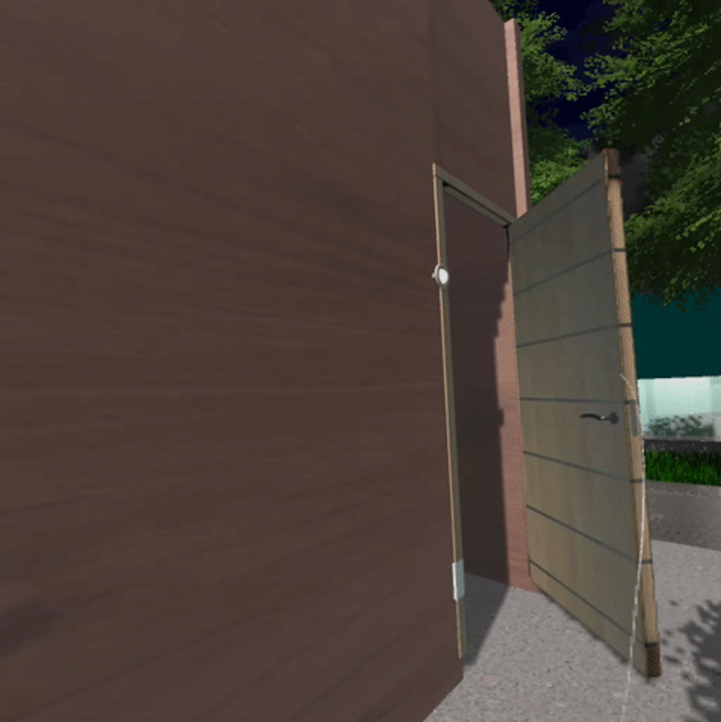
\includegraphics[width=0.45\linewidth]{figures/DoorOpen.png}}
  \subcaptionbox{Closed door.\label{fig:doorclose}}
    {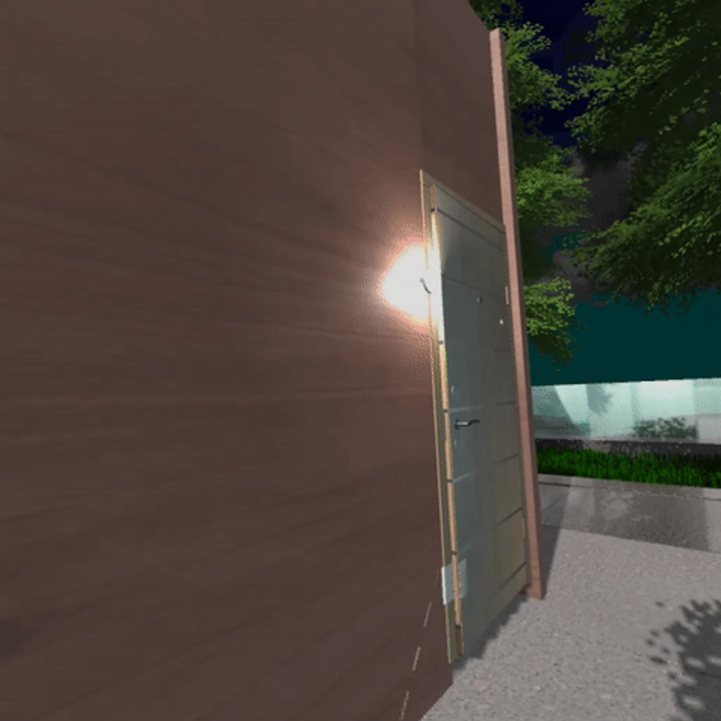
\includegraphics[width=0.45\linewidth]{figures/DoorClose.png}}
  \caption{Door open/close sensor with a light indicator.}
  \label{fig:doorsensor}
\end{figure}

As it was noted, the basic blocks of which the example device consisted are a contact sensor and a switch. As shown in the previous chapter, the platform supports almost all possible Item types presented on the openHAB server. For each item type, there is a corresponding basic Widget. There are 11 basic widgets in total (for example, Dimmer Widget (Figure~\ref{fig:DimmerWidgets-figure}) and Color Picker Widget (Figure~\ref{fig:ColorPickerWidget-figure}) are automatically created for Dimmer and Color Items, respectively). 

\begin{figure}
  \centering
  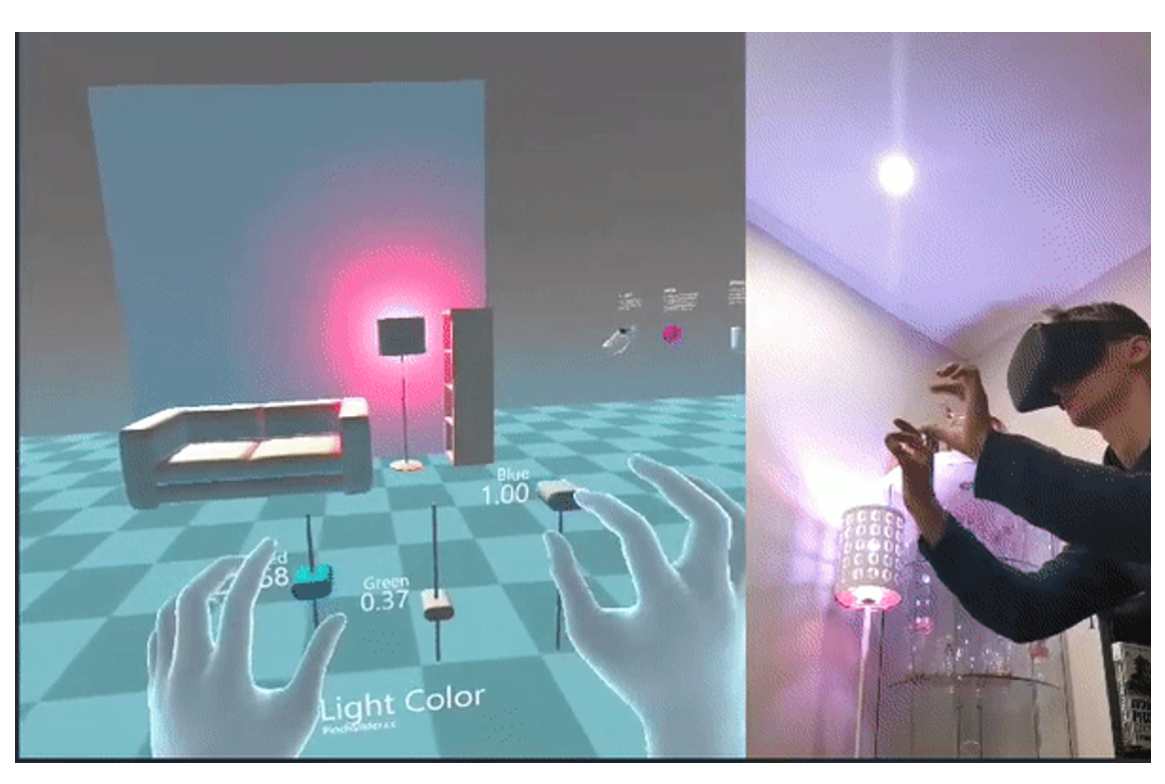
\includegraphics[width=0.9\linewidth]{figures/DimmerWidgets.png}
  \caption{Dimmer Widgets being used to control Red, Green and Blue components of the light.}
  \label{fig:DimmerWidgets-figure}
\end{figure}

\begin{figure}
  \centering
  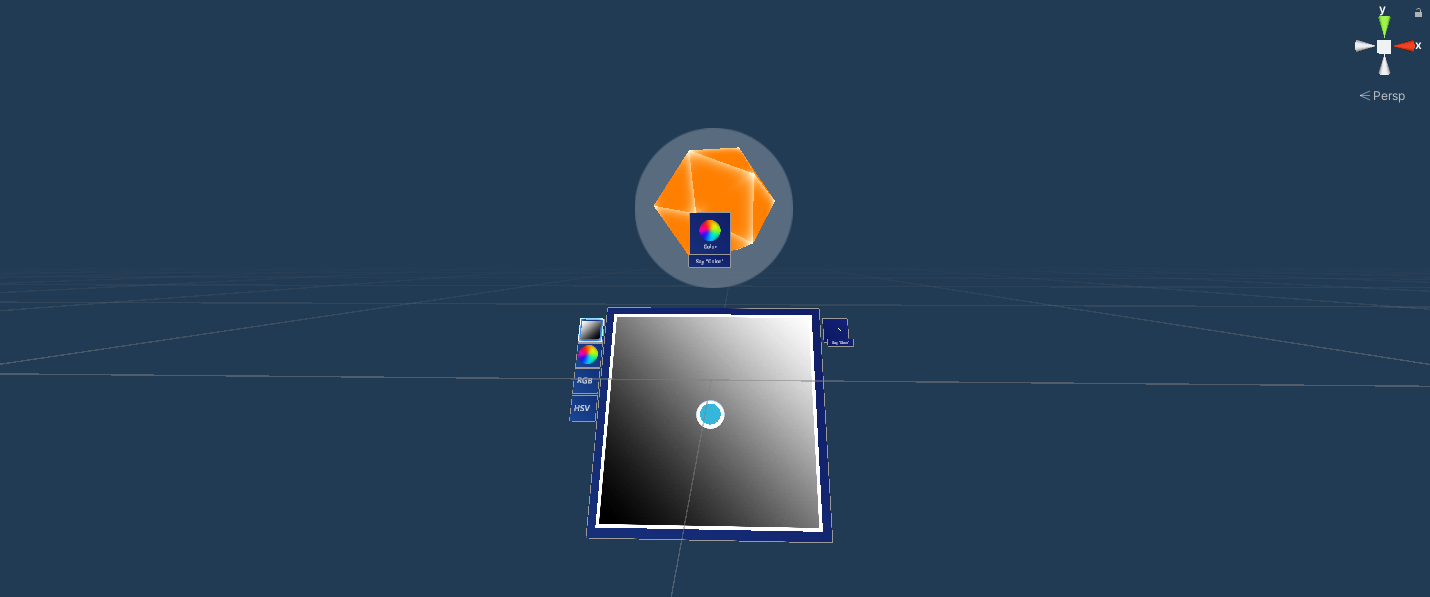
\includegraphics[width=0.9\linewidth]{figures/ColorPickerWidget.png}
  \caption{Color Picker Widget Game Object Prefab. Can select and visualize the Color Item in RGB and HSV formats.}
  \label{fig:ColorPickerWidget-figure}
\end{figure}

For new ways of interacting with IoT devices, tag-based Widgets can be added to an Item. Widgets such as Pressure sensor, Gesture sensor, Audio and Video streaming sensors, Sight sensor expand the possibilities of interaction with devices in virtual reality and are also used to simulate real-life interactive elements. At the moment, there are 12 tag-based Widgets in the NUIX-Studio Development kit. 

For different IoT scenarios, these tag-based Widgets can perform various functions. The platform provides three different environments: Smart Driving, Smart Classroom, and Smart Home environments. In the example scenario, the smartphone changes its mode based on the environment it is located in at the moment. Developers can create their own devices using the Thing Designer tool, and the platform will automatically understand in which environment the device is currently located and adjust its functionality to the given environment. 

\begin{figure}
  \centering
  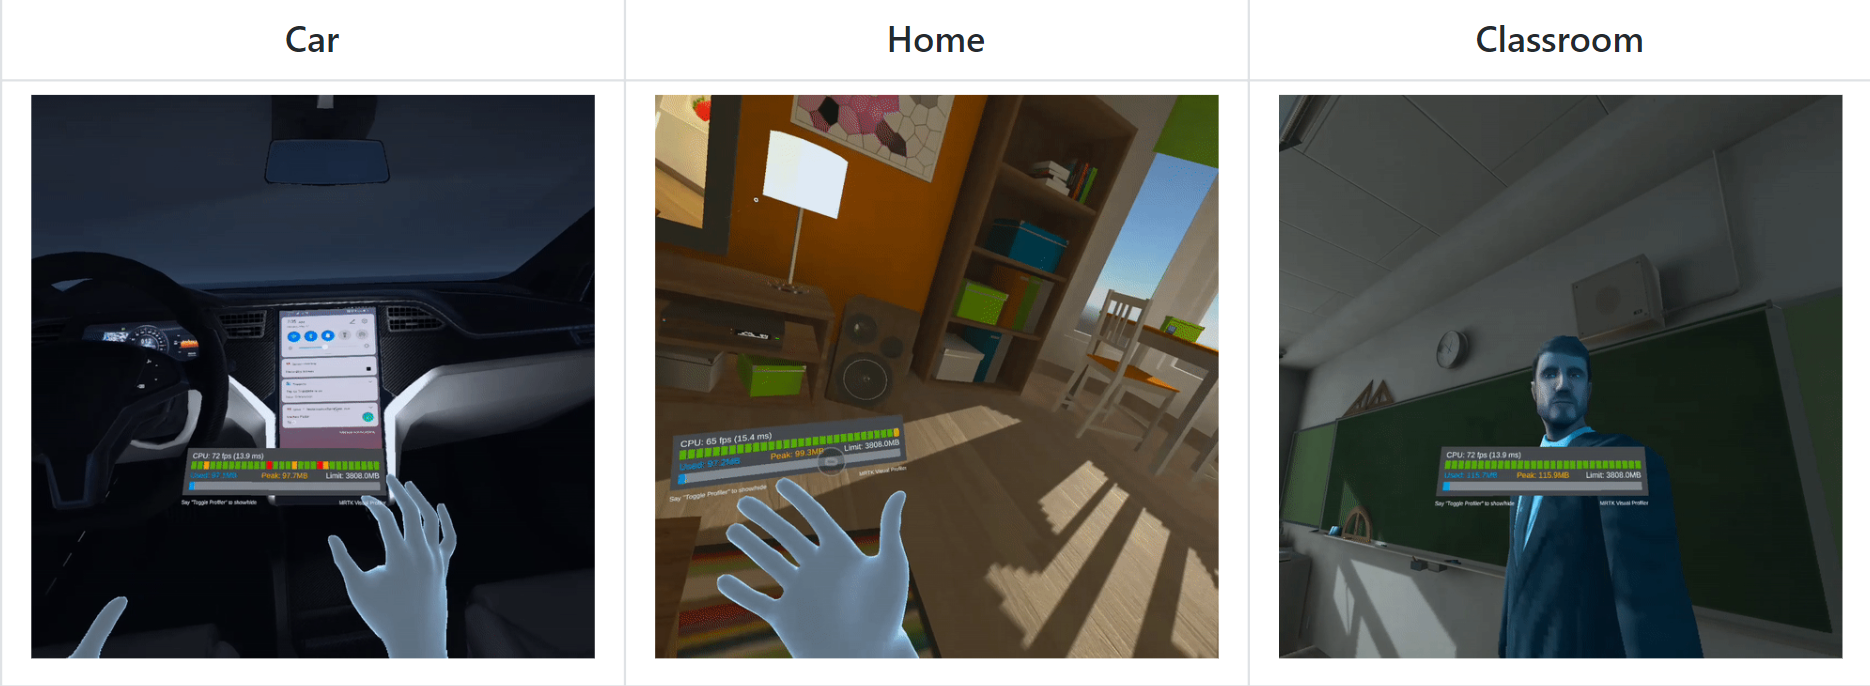
\includegraphics[width=0.9\linewidth]{figures/Environments.png}
  \caption{Three different environments that can be used by developers.}
  \label{fig:Environments-figure}
\end{figure}

\section{Complex computations API}

With the transfer of resource-intensive calculations to a separate server, it becomes possible to perform more reliable physical object simulations. Computations such as processing light, sound, and electromagnetic waves of other frequencies and various substances such as gas, water, are only limited by existing algorithms. 

Storing important physical parameters is sometimes critical for prototyping AIoT projects. For example, the next chapter shows how computing lighting on a separate instance can dramatically improve the user experience. Developers are provided with a tool for storing and synchronizing data for computing physics on the server. Thus, each of the instances can use the result of the computations while using the device's resources only for displaying them. 

\section{API and tools for IoT data visualization and analysis}

Each of IoT devices is visualized through Widgets, but designing Widgets by 3D modeling requires additional time. If a 3D model of the device already exists, the researcher can add it to the platform as a Widget and then connect extra Widgets to it. However, in the IoT environment used, not every device has a corresponding 3D model. There are several solutions to this problem. The first solution is to use 3D models of similar devices. Yet, it is not always possible to find the particular model, or sometimes the quality of these models does not meet the requirements. The second solution is device scanning. With the help of 3D scanners based on depth cameras, it is already possible to scan things with acceptable accuracy and at a relatively affordable price. If millimeter precision scanning is required, then expensive professional solutions can be used.

The resulting Widgets of 3D models can be added to Virtual reality. In the case of the NUIX-Studio App, scenes representing different environments are used. Scenes can be created within Unity editor and by using the Things designer,  or by interpreting the surrounding objects as Widgets (for example, people's position on the street is represented as an Item of Location type). This approach takes a long time to construct a scene, especially if one needs to use a copy of the real environment in Virtual reality. To reduce the time spent on 3D modeling, researchers can use solutions such as 3D scanning of the environment (Figure~\ref{fig:RoomScan-figure}). It is possible to scan the environment with good accuracy on many different smartphones using Depth Lab from Google (Figure~\ref{fig:Object_placement-figure}) and with excellent accuracy on the iPhone using Apple ARKit~\cite{baek_two-dimensional_2020, breitbarth_measurement_2019}. However, these scans of the environment are static scenes. If an object inside this environment is moved, then the scan will have to be performed again. Unfortunately, there is currently no solution to this problem. However, in the next chapter, it will be shown that the platform can be adapted to work with augmented reality, thus eliminating the need to match the real world with the virtual one fully.


\begin{figure}
  \centering
  \subcaptionbox{Depth Lab provides a functionality of placing virtual objects in real world. NUIX-Studio development kit provides API for exporting the Virtual Game Objects into Depth lab to visualize them in real world.\label{fig:Object_placement-figure}}
    {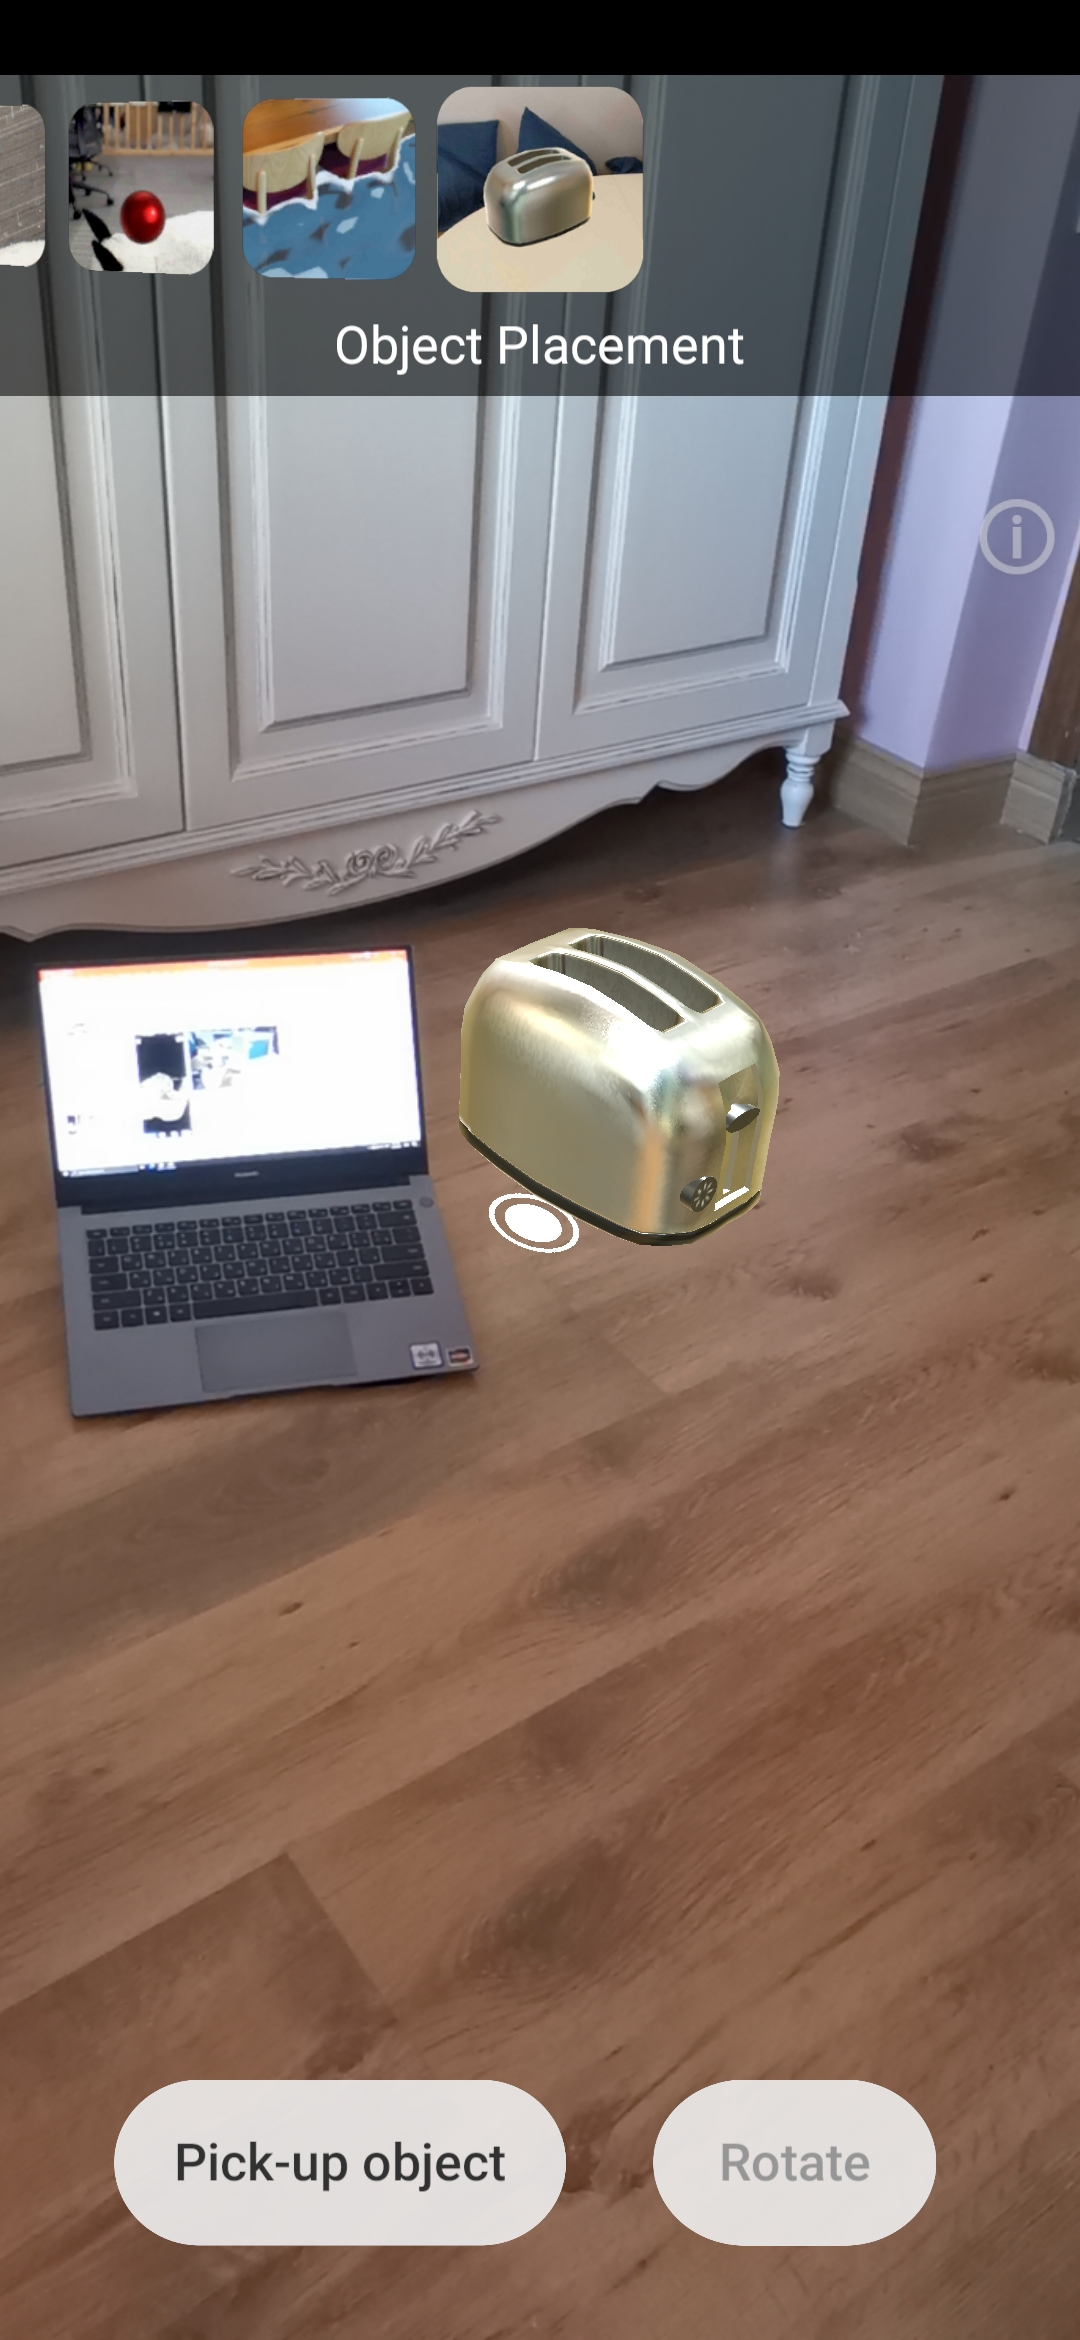
\includegraphics[width=0.45\linewidth]{figures/Object_placement.jpg}}
  \subcaptionbox{3D Scan of a room performed on the Huawei Phone. It can be seen that the scan quality is not ideal.\label{fig:RoomScan-figure}}
    {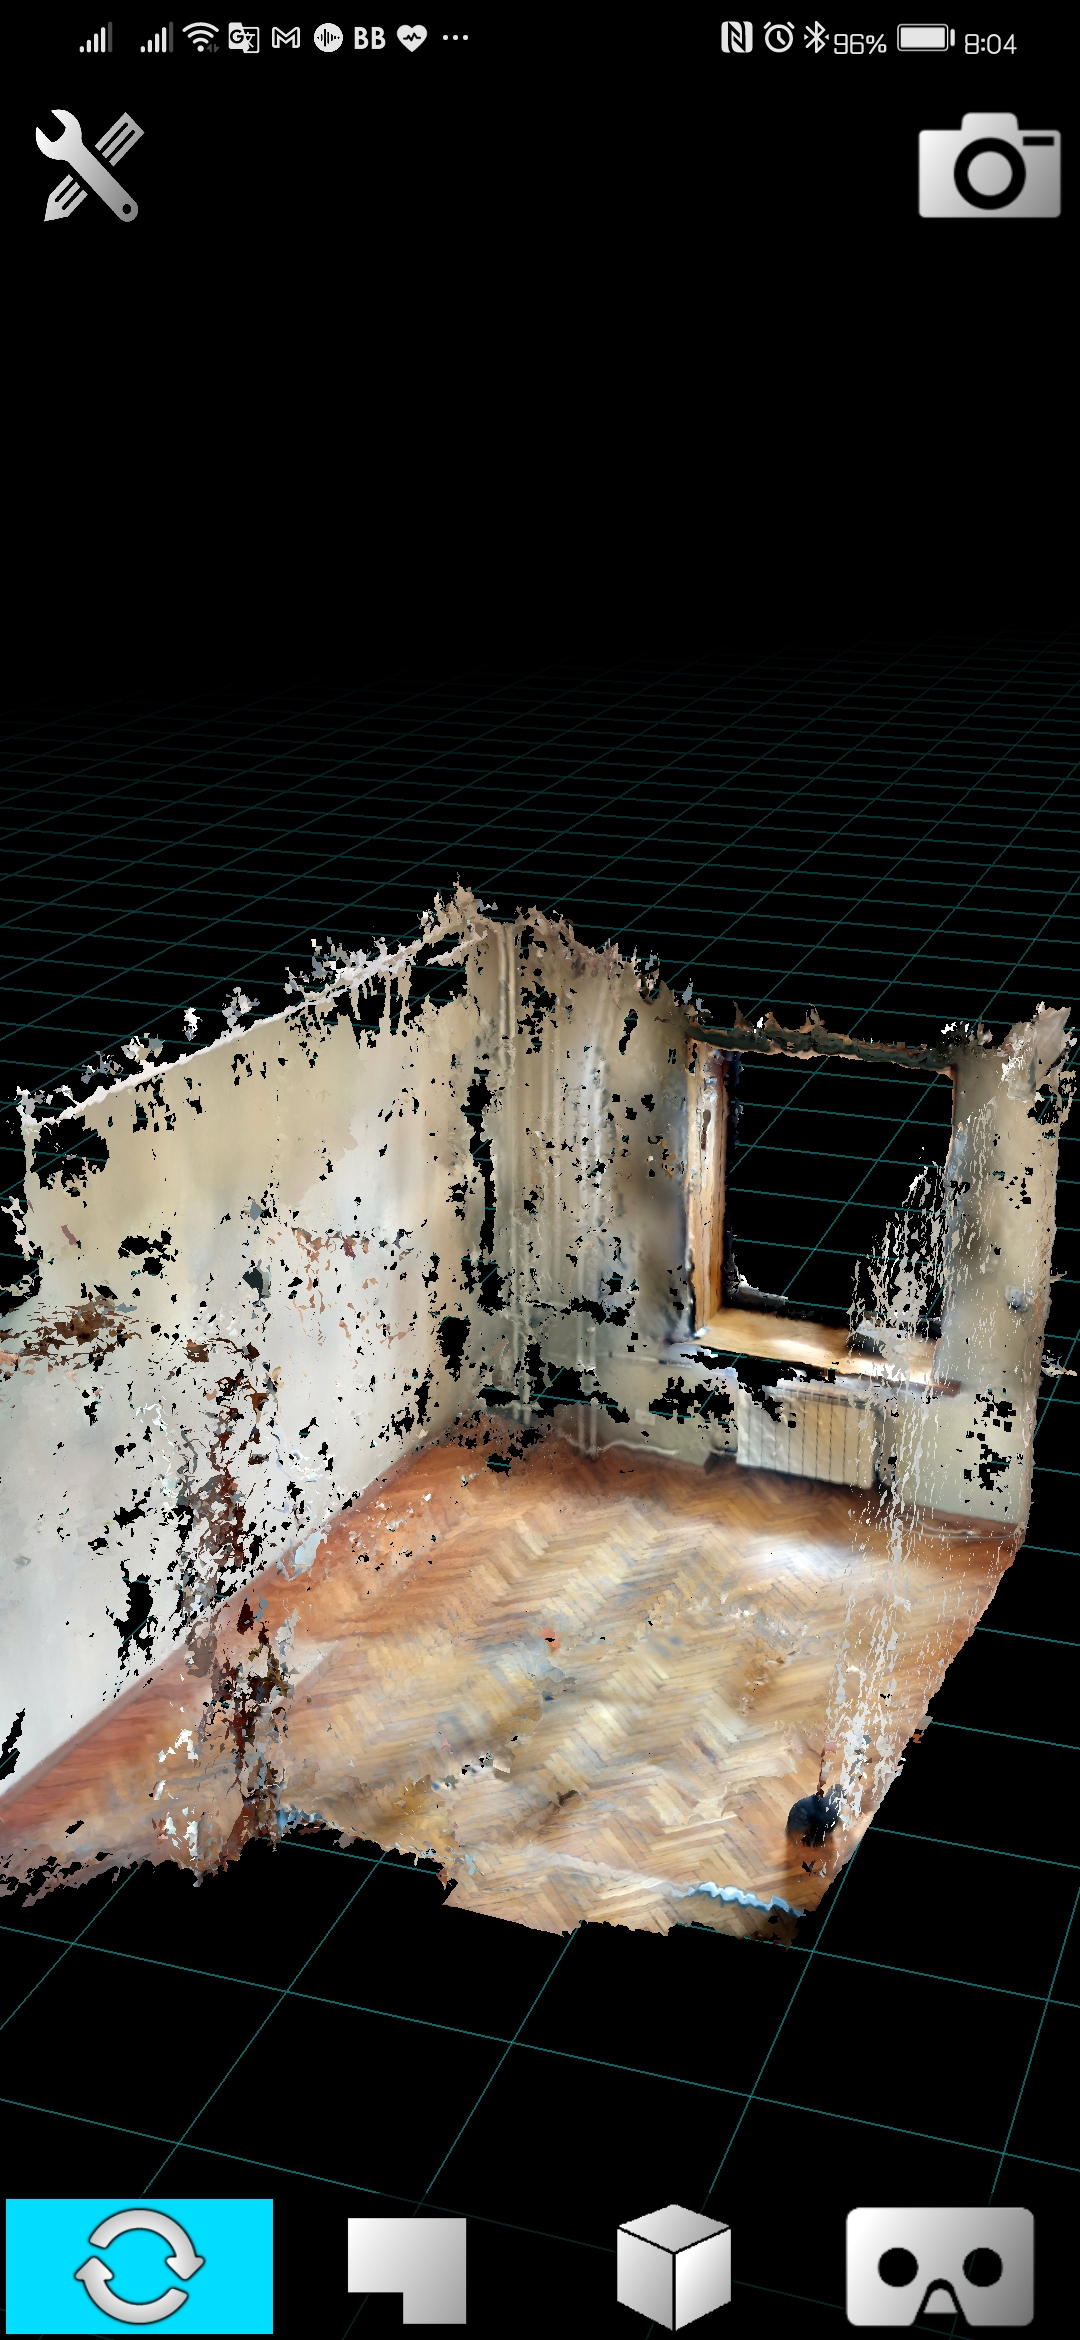
\includegraphics[width=0.45\linewidth]{figures/RoomScan.jpg}}
  \caption{Real world 3D scanning for extending it with virtual devices.}
  \label{fig:exp-screenshot}
\end{figure}

Various devices can track the movement of real IoT devices in the real world, such as Bluetooth tags, QR codes, magnetic field sensors, etc. Researchers can use the API to change the position of each Widget. Thus, when the device's position in the real world changes, the device's Widgets position in the virtual world will also change. It is also possible to perform the opposite action, but this requires a device that will move IoT devices in the real world.

Since changes in Items values are periodically written to the server, they can be visualized using the built-in system tools (Figure~\ref{fig:PersistenceExample-figure}) or further analyzed using external frameworks providing useful insights.

\begin{figure}
  \centering
  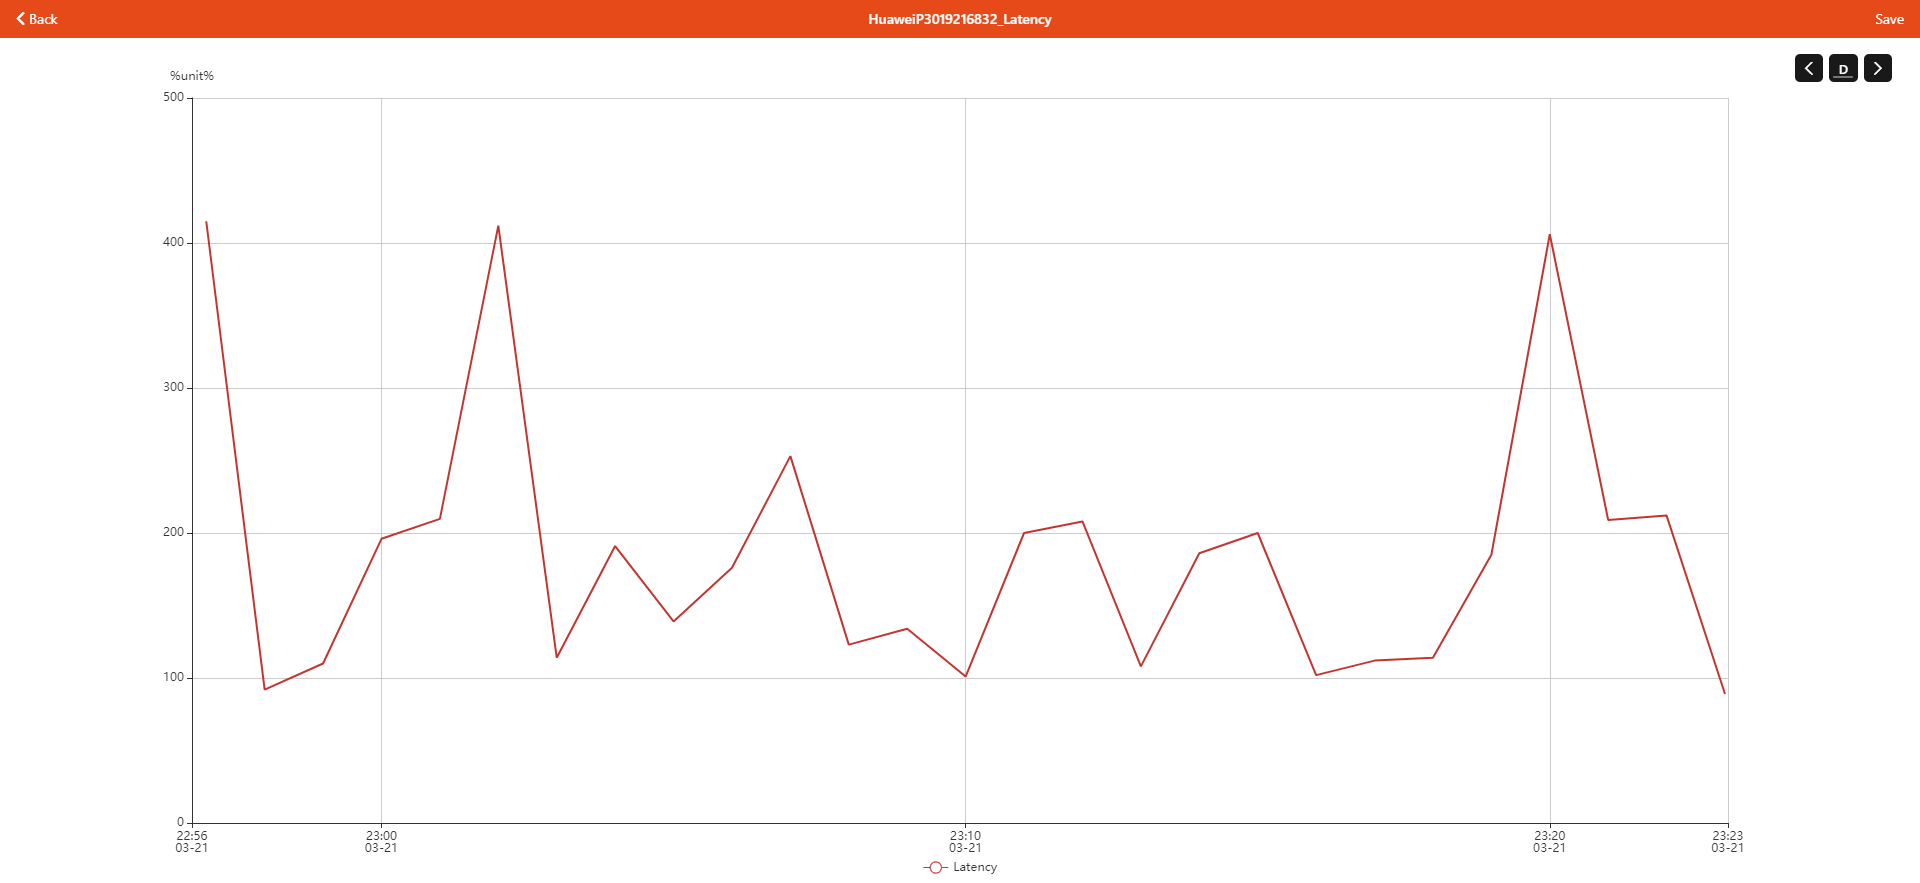
\includegraphics[width=0.9\linewidth]{figures/PersistenceExample.png}
  \caption{Persistence example: Latency value for accessing a remote device (in ms). }
  \label{fig:PersistenceExample-figure}
\end{figure}

\section{API for creating Widgets}

The platform provides only basic Widgets for the Items. These Widgets are used to give an example of how to visualize the IoT devices' data. By using this API, researchers can create Widgets specific to the device they develop. However, most of the Widgets to be developed can be divided into two categories: Sensor Widgets and Visual Widgets.

A virtual sensor Widget has been developed already. By using this Widget, researchers only need to build functions that will activate this sensor. Thus, the time spent on developing widgets is significantly reduced. In addition, the platform provides access to a large number of UX building blocks using the Mixed Reality Toolkit. Using this toolkit, the user will not need to spend time designing various buttons and switches. 


\begin{figure}
  \centering
  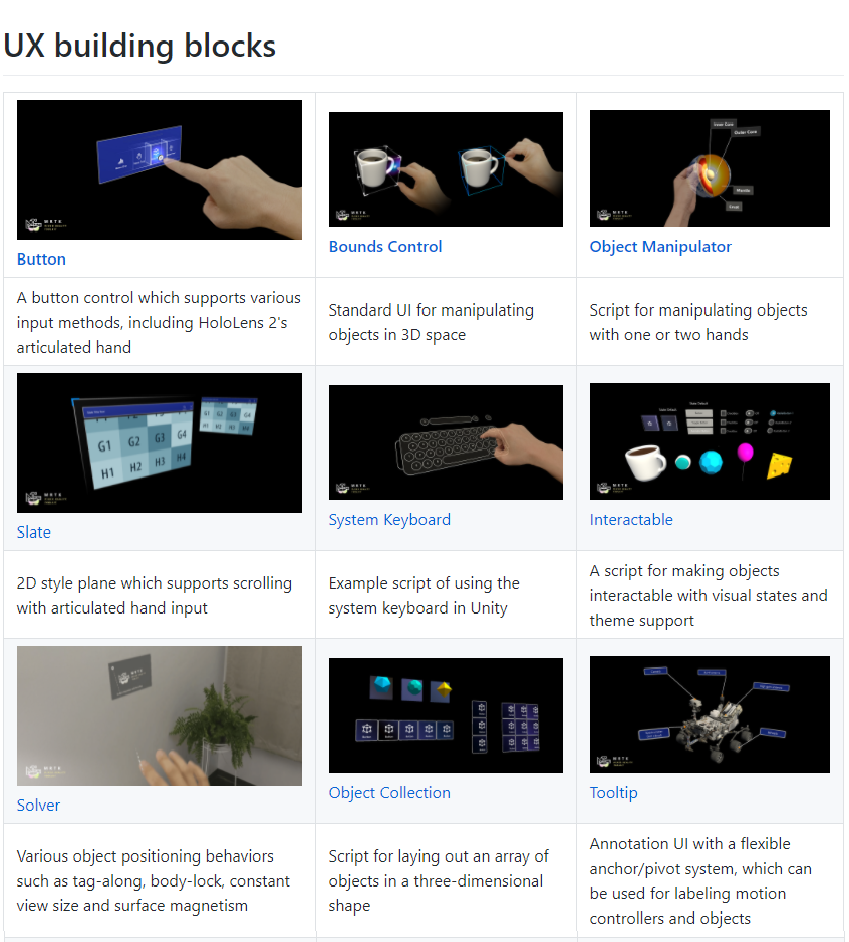
\includegraphics[width=0.6\linewidth]{figures/MRTK.png}
  \caption{UX building blocks.}
  \label{fig:MRTK-figure}
\end{figure}

\section{Summary}

With the help of the NUIX-Studio development kit, researchers can already create prototypes of projects for various AIoT scenarios. The toolkit provides a wide range of different widgets for developing new devices in virtual reality. In addition, the platform helps researchers to connect them with real-world devices in a relatively short time. Additionally, the platform allows developers to receive and send data to various AR applications. As a result, the developer can carry out an entire cycle of prototyping projects with a minimum investment of time and effort into development.
% !TeX root = ../thuthesis-example.tex

\chapter{Platform performance evaluation}

% !TeX root = ../thuthesis-example.tex

\chapter{Platform application}

% !TeX root = ../thuthesis-example.tex

\chapter{\MakeUppercase{Conclusion}}


\section{Future directions}

A possible NUIX-Studio development timeline was created. As seen in Figure~\ref{fig:Timeline-figure}, the development started with providing support for Virtual reality headsets. The next step was implementing openHAB and database support to perform simultaneous interaction in the same environment across several App instances. However, the Things designer is not fully developed since further research is needed to provide a wider variety of supported Widgets.

\begin{figure}
  \centering
  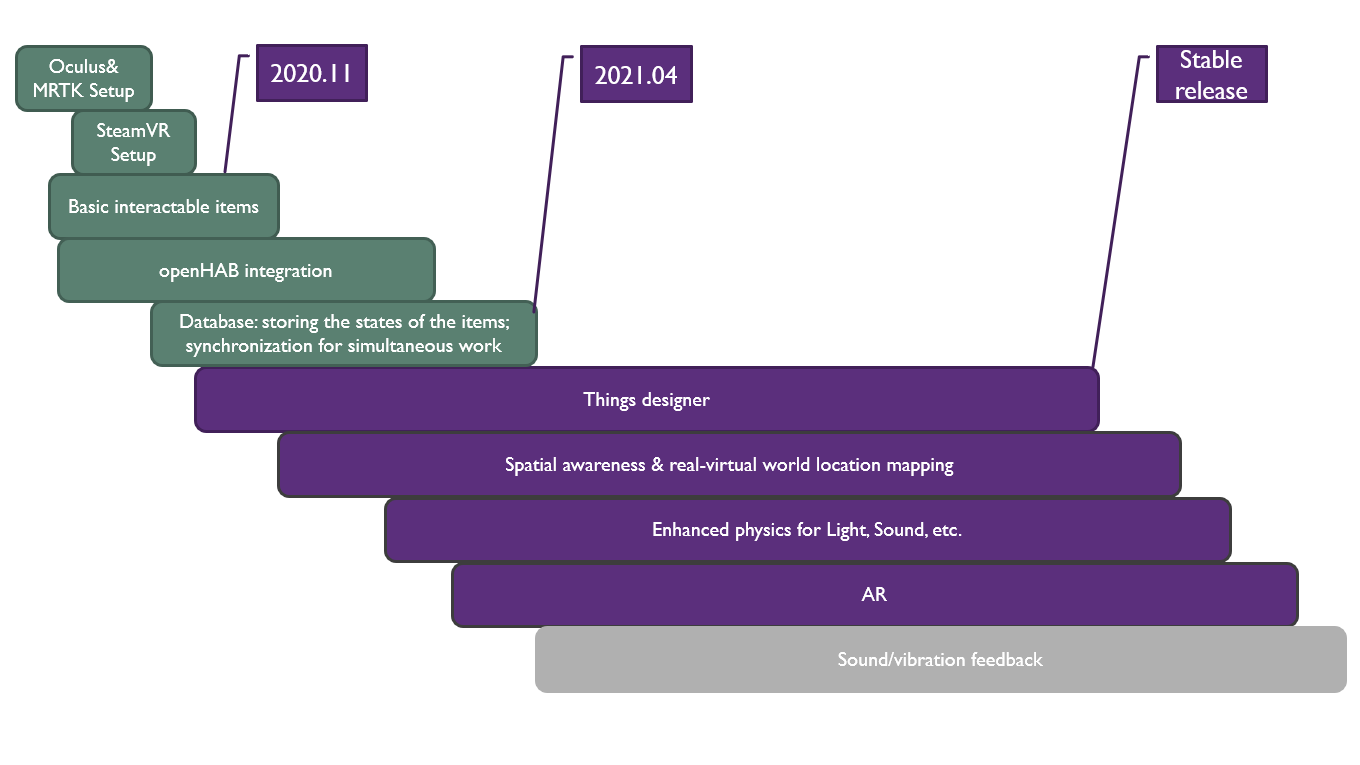
\includegraphics[width=0.9\linewidth]{figures/Timeline.png}
  \caption{Timeline for NUIX-Studio platform development. Green indicates that the task has been developed, purple indicates that the task development has been started, and grey indicates that it has not yet been started.}
  \label{fig:Timeline-figure}
\end{figure}

The Mixed Reality toolkit can provide real-world environmental awareness for apps running on Hololens. It is already possible to run the NUIX-Studio App on Hololens, although it has not been tested yet. Using spatial awareness, the NUIX-Studio App will be able to align virtual Widgets onto IoT devices. Developing real-virtual world location mapping for the Widgets in Virtual reality will be required as well.

Currently, only advanced illumination can be computed on the NUIX-Studio APP. Researchers may need more accurate data to create new IoT devices. In this case, Unity Game Engine can be extended with more precise light, sound, and other physics support.

Enabling AR support requires adding new interaction techniques and training Deep learning models to provide object recognition. Users can use both AR and VR to research new IoT devices, with AR being responsible for retrieving the coordinates of the devices from the real world (by OpenCV, Tensoflow Graphics, etc.), and VR for visualizing environments that are difficult or impossible to implement in AR (for example, flying on a plane or driving a car).

Augmented reality, Virtual reality, and Mixed Reality are not the only interfaces to interact with IoT in the virtual world. What if the feedback from IoT devices is provided only by sound and vibrations? The NUIX-Studio can be adapted for such limitations. One of the examples of this approach is research for visually impaired people in an IoT environment.

NUIX-Studio is distributed through Github repository~\cite{NUIXStudio}. The future releases and tutorials will be posted there (Figure~\ref{fig:GitHub-figure}). The final version of NUIX-Studio is expected to be released once the Thing Designer functionality is fully developed. The author welcomes researchers' help, but only one contribution to the code of NUIX-Studio has been made by another student, with the rest of the platform code created by the author.


\begin{figure}
  \centering
  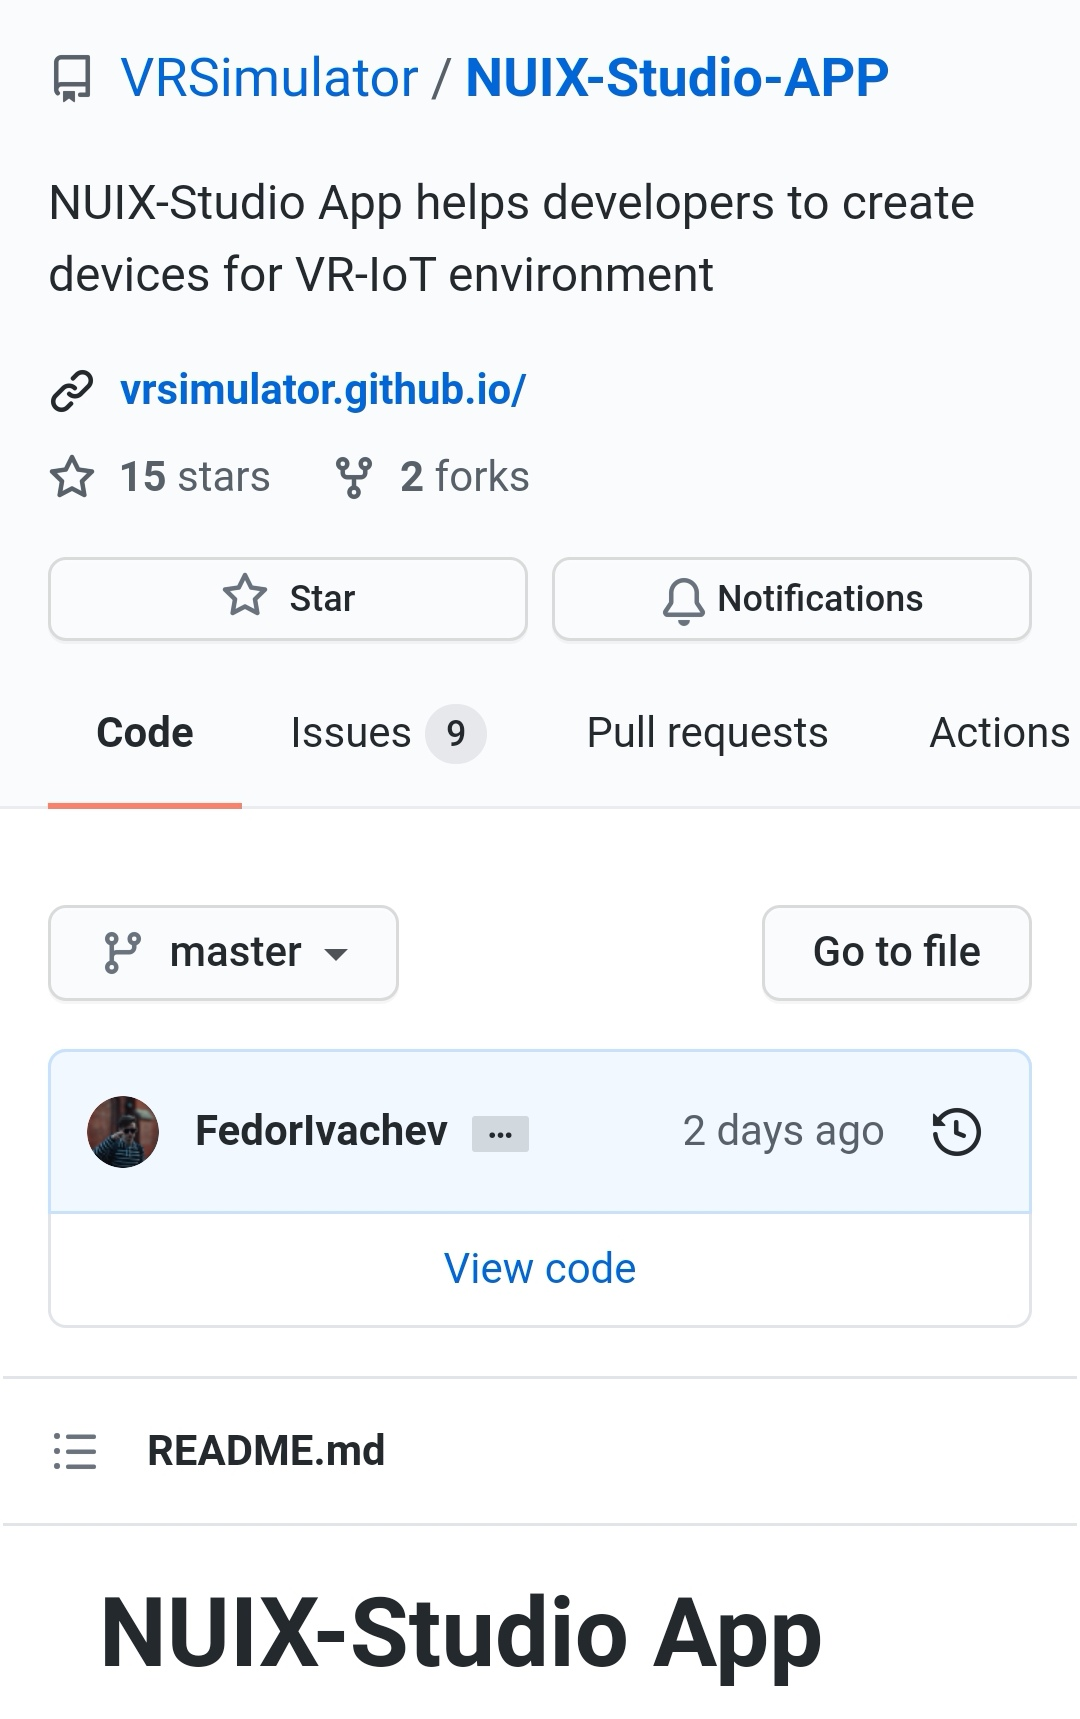
\includegraphics[width=0.6\linewidth]{figures/GitHub.jpg}
  \caption{The front page of the NUIX-Studio Github repository.}
  \label{fig:GitHub-figure}
\end{figure}

\section{Summary}

The result of the research is a developed concept of the platform, as well as the basis for further development of tools for creating IoT devices in Virtual, Augmented and Mixed reality. By creating a prototype platform, the following hypothesis have been proven:

\begin{enumerate}
    \item Using the presented architecture, any IoT device can be added to the virtual world;
    \item It is possible to add new functionality to existing IoT devices inside the VR environment;
    \item It is possible to create completely virtual devices and embed them in the same environment with real devices;
    \item The synchronization time between devices within the IoT-VR environment is currently limited by the network speed;
    \item It is possible for several users to work simultaneously in one IoT-VR environment;
    \item To improve user experience, it is necessary to separate data and interaction calculation tasks between different application instances;
    \item The platform is scalable;
\end{enumerate}


The developed solution has the following advantages:\footnote{Considering that there are no similar solutions on the market, these advantages can be considered a reserve for the future}
\begin{enumerate}
    \item Integration of third-party solutions is possible both from the IoT support side and from the VR side;
    \item The platform's implementation is lightweight and is not based on many third-party frameworks;
    \item The development team can add new members without the need to teach people new technologies since the main part of the platform is written in C\# inside the Unity engine. It also has the advantage of more conveniently adding external projects into the platform;
    \item Researchers can use the platform API to create elements of interaction with IoT devices;
    \item A tool called Thing designer allows researchers to create new IoT devices using both VR and the Web interface;
    \item A tool is being developed to track the position of real devices and synchronize with their position in the virtual world (can start from using QR-codes);
    \item It is shown that the platform is capable of working not only with Virtual but also with Augmented and Mixed reality, and simultaneous operation of each reality-based App within the same IoT environment is possible;
    \item It is shown that the platform provides support for complex physical computations.
\end{enumerate}

Nevertheless, there are still limitations associated with creating a complete copy of the real-world environment inside the virtual one, particularly surrounding the need to manually add movable objects in the form of Items and Widgets.

The author hopes that this research will form the basis of a product that will have a significant value in the future, allowing the creation of new devices, including those for use in new generation networks.


% 其他部分 
\backmatter

% 参考文献

\bibliography{references, ref/refs}  % 参考文献使用 BibTeX 编译
%\printbibliography       % 参考文献使用 BibLaTeX 编译

% 附录
%\appendix
%% !TeX root = ../thuthesis-example.tex

%\chapter{Supplementary material}



% \section{Visualization of Attention Weights}

% These experiments aim to analyse some inner properties of the model that were not shown in the paper:
% \begin{itemize}[noitemsep,topsep=0pt,parsep=0pt,partopsep=0pt]
% 	\item Vizualize at each stack of the encoder how the self attention change for regular image
% 	\item Case of occlusion of two predictions how are the attention maps: For example, how the attention of enc and dec change with depth in order to find the self-att of the same object and how slot coordinates their duties with each other and then changes the picture to high occlusion, iou $> 0.7$ object diagram, to see if self-attention runs to the nearby object in the case of high occlusion.
% 	\item Vizualize at each stack of the decoder: Eventhough initially each object queries are responsible for many zones, at the last layer each slot has an attention for a single object, that means that at each stacking decoder each object queries will correct its spatial attention.
% \end{itemize}

% Note: we extract attention weights averaged over all heads. Attention weights are given by the following vectorized formula $softmax(\frac{QK^{T}}{\sqrt{d_{k}}})$. On these experience we show attention weights for each object of the image. We use 8 multi attention heads and 6 layers for both encoder and decoder.

% \subsection{Attention weights on encoder}
% Hooks are used to extract output of each layers of the decoder, their shape is $[N, L, L]$ with $N$ the batch size, and $L$ the size of the last feature map. Hence we get a relative attention weight w.r.t to each point. 
% \begin{figure}[!htbp]
% 	\centering
% 	\includegraphics[scale=0.25]{images/1st_layer.png}
% 	\caption{first layer}
% \end{figure}
% \FloatBarrier

% \begin{figure}[!htbp]
% 	\centering
% 	\includegraphics[scale=0.25]{images/2nd_layer.png}
% 	\caption{second layer}
% \end{figure}
% \FloatBarrier

% \begin{figure}[!htbp]
% 	\centering
% 	\includegraphics[scale=0.25]{images/3rd_layer.png}
% 	\caption{third layer}
% \end{figure}
% \FloatBarrier

% \begin{figure}[!htbp]
% 	\centering
% 	\includegraphics[scale=0.25]{images/4th_layer.png}
% 	\caption{fourth layer}
% \end{figure}
% \FloatBarrier

% \begin{figure}[!htbp]
% 	\centering
% 	\includegraphics[scale=0.25]{images/5th_layer.png}
% 	\caption{fifth layer}
% \end{figure}
% \FloatBarrier

% \begin{figure}[!htbp]
% 	\centering
% 	\includegraphics[scale=0.25]{images/6th_layer.png}
% 	\caption{last layer}
% \end{figure}
% \FloatBarrier

% We can observe that at each layer the encoder seperates the two cat instances, the first layer is outputs near random attentions, then the 2nd and 3rd layers detects the two cats instances, and in the fourth layer the encoder seperate the instances. 


% \begin{figure}[!htbp]
% 	\centering
% 	\includegraphics[scale=0.25]{images/enc1.png}
% 	\caption{first layer}
% \end{figure}
% \FloatBarrier

% \begin{figure}[!htbp]
% 	\centering
% 	\includegraphics[scale=0.25]{images/lastenc.png}
% 	\caption{last layer}
% \end{figure}
% \FloatBarrier

% \subsection{Attention weights on decoder}
% Hooks are used to extract output of each layers of the decoder, their shape is $[N, S, L]$ with $N$ the batch size, $S$ the number of object queries and $L$ the size of the last feature map. 
% \begin{figure}[!htbp]
% 	\centering
% 	\includegraphics[scale=0.25]{images/first_layer.png}
% 	\caption{first layer}
% \end{figure}
% \FloatBarrier

% \begin{figure}[!htbp]
% 	\centering
% 	\includegraphics[scale=0.25]{images/second_layer.png}
% 	\caption{second layer}
% \end{figure}
% \FloatBarrier

% \begin{figure}[!htbp]
% 	\centering
% 	\includegraphics[scale=0.25]{images/third_layer.png}
% 	\caption{third layer}
% \end{figure}
% \FloatBarrier

% \begin{figure}[!htbp]
% 	\centering
% 	\includegraphics[scale=0.25]{images/fourth_layer.png}
% 	\caption{fourth layer}
% \end{figure}
% \FloatBarrier



% \begin{figure}[!htbp]
% 	\centering
% 	\includegraphics[scale=0.25]{images/fifth_layer.png}
% 	\caption{fifth layer}
% \end{figure}
% \FloatBarrier


% \begin{figure}[!htbp]
% 	\centering
% 	\includegraphics[scale=0.25]{images/decoder_last_layer.png}
% 	\caption{last layer}
% \end{figure}
% \FloatBarrier

% We can see that our model mostly is able to attend the edges of the object directly after the first layer this might be due to the fact that the encoder has already seperated the different instances. 


% \subsection{Attention weights on high occlusion objects}
% Note: I tried a lot of pictures with a lot of objects with high occlusion most of the time the model performed poorly (e.g 1 or 2 false positive that have high occlusion). On this experience query 27 (first prediction) is a prediction with very low probablity (0.1) from the model. For the encoder attention weights relative to the top two points are shown on the left, and the bottom two points are shown on the right.

% \begin{figure}[!htbp]
% 	\centering
% 	\includegraphics[scale=0.23]{images/encoder_1st.png}
% 	\caption{first layer encoder}
% \end{figure}
% \FloatBarrier


% \begin{figure}[!htbp]
% 	\centering
% 	\includegraphics[scale=0.23]{images/encoder_2nd.png}
% 	\caption{second layer encoder}
% \end{figure}
% \FloatBarrier


% \begin{figure}[!htbp]
% 	\centering
% 	\includegraphics[scale=0.23]{images/encoder_3rd.png}
% 	\caption{third layer encoder}
% \end{figure}
% \FloatBarrier


% \begin{figure}[!htbp]
% 	\centering
% 	\includegraphics[scale=0.23]{images/encoder_4th.png}
% 	\caption{fourth layer encoder}
% \end{figure}
% \FloatBarrier


% \begin{figure}[!htbp]
% 	\centering
% 	\includegraphics[scale=0.23]{images/encoder_5th.png}
% 	\caption{fifth layer encoder}
% \end{figure}
% \FloatBarrier


% \begin{figure}[!htbp]
% 	\centering
% 	\includegraphics[scale=0.23]{images/encoder_6th.png}
% 	\caption{last layer encoder}
% \end{figure}
% \FloatBarrier




% \begin{figure}[!htbp]
% 	\centering
% 	\includegraphics[scale=0.23]{images/decoder_1st.png}
% 	\caption{first layer decoder}
% \end{figure}
% \FloatBarrier




% \begin{figure}[!htbp]
% 	\centering
% 	\includegraphics[scale=0.23]{images/decoder_2nd.png}
% 	\caption{second layer decoder}
% \end{figure}
% \FloatBarrier




% \begin{figure}[!htbp]
% 	\centering
% 	\includegraphics[scale=0.23]{images/decoder_3rd.png}
% 	\caption{third layer decoder}
% \end{figure}
% \FloatBarrier





% \begin{figure}[!htbp]
% 	\centering
% 	\includegraphics[scale=0.23]{images/decoder_4th.png}
% 	\caption{fourth layer decoder}
% \end{figure}
% \FloatBarrier




% \begin{figure}[!htbp]
% 	\centering
% 	\includegraphics[scale=0.23]{images/decoder_5th.png}
% 	\caption{fifth layer decoder}
% \end{figure}
% \FloatBarrier




% \begin{figure}[!htbp]
% 	\centering
% 	\includegraphics[scale=0.23]{images/decoder_6th.png}
% 	\caption{last layer decoder}
% \end{figure}
% \FloatBarrier


% We can see a similar behaviour for object with high occlusion, the decoder does not rectify its bounding box and is able at the first layer to decide the object is by attending its edge using information from the encoder. Also we can see that query 27 and 71 are duplicate predictions somehow the model is able to predict a low probability for the query 27 and predict query 71 with confidence. Moreover looking at the prediction of each object queries we can see that almost all of them are predicting the class Elephant somehow the model is able to chose the object queries that has the best bounding box with high confidence while their attention weights seems to stay identical between each layer. \\
% We can clearly observe that stacking encoding layers are essential as the first layers predict random instances, and last layers are able to separate instances. On the other hand, the decoder seems to not change its attention weights at each stack, but the paper states significant increase in AP as it stacks more layers on the decoder. Perhaps we should look at the attentions on the the object queries instead of the decoder?

% \subsection{Attention weights on object queries}

% Hooks are used to extract output of self attention of the object queries at each layers of the decoder, their shape is $[N, S, S]$ with $N$ the batch size and $S$ the number of object queries. In this experience we take relative weights for object queries 1, 2, 3, \textbf{27, 71, 92}, 93, 94, 95. Object queries \textbf{27, 71, 92} are prediction with confidence $> 0.1$, the rest are chosen to be object query that should not influence the predictions of \textbf{27, 71, 92}, as they do not involve occlusion or duplicate predictions. Object queries are shown in the same order in the figures. 

% \begin{figure}[!htbp]
% 	\centering
% 	\includegraphics[scale=0.23]{images/query_1st.png}
% 	\caption{first layer object queries}
% \end{figure}
% \FloatBarrier


% \begin{figure}[!htbp]
% 	\centering
% 	\includegraphics[scale=0.23]{images/query_2nd.png}
% 	\caption{second layer object queries}
% \end{figure}
% \FloatBarrier


% \begin{figure}[!htbp]
% 	\centering
% 	\includegraphics[scale=0.23]{images/query_3rd.png}
% 	\caption{third layer object queries}
% \end{figure}
% \FloatBarrier


% \begin{figure}[!htbp]
% 	\centering
% 	\includegraphics[scale=0.23]{images/query_4th.png}
% 	\caption{fourth layer object queries}
% \end{figure}
% \FloatBarrier


% \begin{figure}[!htbp]
% 	\centering
% 	\includegraphics[scale=0.23]{images/query_5th.png}
% 	\caption{fifth layer object queries}
% \end{figure}
% \FloatBarrier


% \begin{figure}[!htbp]
% 	\centering
% 	\includegraphics[scale=0.23]{images/query_6th.png}
% 	\caption{last layer object queries}
% \end{figure}
% \FloatBarrier


% Object queries  \textbf{27, 71, 92} are prediction with high occlusion and object queries  \textbf{27, 71} are duplicate prediction. Hence we expect their attention weights to be higher. The results validate our hypothesis, indeed at the first and second layers we can see that the object queries attend random object queries, and at the last three layers, object query \textbf{27} only attend its duplicate \textbf{71}, and we can see that object query \textbf{92} also mostly attends object query \textbf{71} which are two predictions with high occlusion. \\
% In previous experiences it seemed like the decoder did not change its attention weights at each stack, instead it changed its attention weights at the object query level.


% \subsection{Single Encoder Double Decoder}


% These experiences aim to explore how the attention mechanism works for classification and regression, both task have their decoder and share an encoder. We note for the same length of training a drop of 0.1 in AP
% \begin{itemize}[noitemsep,topsep=0pt,parsep=0pt,partopsep=0pt]
% 	\item Visualize attention on decoder1 for classification
% 	\item Visualize attention on decoder2 for regression
% \end{itemize}

% \subsubsection{Decoder classification}

% \begin{figure}[!htbp]
% 	\centering
% 	\includegraphics[scale=0.2]{images/decoder_cls_first.png}
	
% 	\caption{Classification Layer 1}
% \end{figure}
% \FloatBarrier



% \begin{figure}[!htbp]
% 	\centering
% 	\includegraphics[scale=0.2]{images/decoder_cls_second.png}
	
% 	\caption{Classification Layer 2}
% \end{figure}
% \FloatBarrier




% \begin{figure}[!htbp]
% 	\centering
% 	\includegraphics[scale=0.2]{images/decoder_cls_third.png}
	
% 	\caption{Classification Layer 3}
% \end{figure}
% \FloatBarrier



% \begin{figure}[!htbp]
% 	\centering
% 	\includegraphics[scale=0.2]{images/decoder_cls_fourth.png}
	
% 	\caption{Classification Layer 4}
% \end{figure}
% \FloatBarrier




% \begin{figure}[!htbp]
% 	\centering
% 	\includegraphics[scale=0.2]{images/decoder_cls_fifth.png}
	
% 	\caption{Classification Layer 5}
% \end{figure}
% \FloatBarrier
		

% \begin{figure}[!htbp]
% 	\centering
% 	\includegraphics[scale=0.2]{images/decoder_cls_last.png}
	
% 	\caption{Classification Layer 6}
% \end{figure}
% \FloatBarrier


% \subsubsection{Decoder Regression}

% \begin{figure}[!htbp]
% 	\centering
% 	\includegraphics[scale=0.2]{images/decoder_reg_first.png}
	
% 	\caption{Regression Layer 1}
% \end{figure}
% \FloatBarrier


% \begin{figure}[!htbp]
% 	\centering
% 	\includegraphics[scale=0.2]{images/decoder_reg_second.png}
	
% 	\caption{Regression Layer 2}
% \end{figure}
% \FloatBarrier


% \begin{figure}[!htbp]
% 	\centering
% 	\includegraphics[scale=0.2]{images/decoder_reg_third.png}
	
% 	\caption{Regression Layer 3}
% \end{figure}
% \FloatBarrier


% \begin{figure}[!htbp]
% 	\centering
% 	\includegraphics[scale=0.2]{images/decoder_reg_fourth.png}
	
% 	\caption{Regression Layer 4}
% \end{figure}
% \FloatBarrier



% \begin{figure}[!htbp]
% 	\centering
% 	\includegraphics[scale=0.2]{images/decoder_reg_fifth.png}
	
% 	\caption{Regression Layer 5}
% \end{figure}
% \FloatBarrier
	

% \begin{figure}[!htbp]
% 	\centering
% 	\includegraphics[scale=0.2]{images/decoder_reg_last.png}
	
% 	\caption{Regression Layer 6}
% \end{figure}
% \FloatBarrier



% \subsubsection{Attention on Encoder}

% \begin{figure}[!htbp]
% 	\centering
% 	\includegraphics[scale=0.2]{images/encoder_sedd_first.png}
	
% 	\caption{Layer 1}
% \end{figure}
% \FloatBarrier
	

% \begin{figure}[!htbp]
% 	\centering
% 	\includegraphics[scale=0.2]{images/encoder_sedd_second.png}
	
% 	\caption{Layer 2}
% \end{figure}
% \FloatBarrier



% \begin{figure}[!htbp]
% 	\centering
% 	\includegraphics[scale=0.2]{images/encoder_sedd_third.png}
	
% 	\caption{Layer 3}
% \end{figure}
% \FloatBarrier


% \begin{figure}[!htbp]
% 	\centering
% 	\includegraphics[scale=0.2]{images/encoder_sedd_fourth.png}
	
% 	\caption{Layer 4}
% \end{figure}
% \FloatBarrier


% \begin{figure}[!htbp]
% 	\centering
% 	\includegraphics[scale=0.2]{images/encoder_sedd_fifth.png}
	
% 	\caption{Layer 5}
% \end{figure}
% \FloatBarrier


% \begin{figure}[!htbp]
% 	\centering
% 	\includegraphics[scale=0.2]{images/encoder_sedd_last.png}
	
% 	\caption{Layer 6}
% \end{figure}
% \FloatBarrier



% \subsection{Double Encoder Double Decoder}


% These experiences aim to explore how the attention mechanism works for classification and regression, we use two encoder and two decoders, one for each tasks. We notice a drop of 3pts in AP.
% \begin{itemize}[noitemsep,topsep=0pt,parsep=0pt,partopsep=0pt]
% 	\item Visualize attention on encoder1 for classification
% 	\item Visualize attention on encoder2 for regression
% 	\item Visualize attention on decoder1 for classification
% 	\item Visualize attention on decoder2 for regression
% \end{itemize}

% \subsubsection{Decoder Classification}

% \begin{figure}[!htbp]
% 	\centering
% 	\includegraphics[scale=0.2]{images/decoder_cls_first_0.png}
	
% 	\caption{Layer 1}
% \end{figure}
% \FloatBarrier


% \begin{figure}[!htbp]
% 	\centering
% 	\includegraphics[scale=0.2]{images/decoder_cls_second_0.png}
	
% 	\caption{Layer 2}
% \end{figure}
% \FloatBarrier


% \begin{figure}[!htbp]
% 	\centering
% 	\includegraphics[scale=0.2]{images/decoder_cls_third_0.png}
	
% 	\caption{Layer 3}
% \end{figure}
% \FloatBarrier


% \begin{figure}[!htbp]
% 	\centering
% 	\includegraphics[scale=0.2]{images/decoder_cls_fourth_0.png}
	
% 	\caption{Layer 4}
% \end{figure}
% \FloatBarrier


% \begin{figure}[!htbp]
% 	\centering
% 	\includegraphics[scale=0.2]{images/decoder_cls_fifth_0.png}
	
% 	\caption{Layer 5}
% \end{figure}
% \FloatBarrier


% \begin{figure}[!htbp]
% 	\centering
% 	\includegraphics[scale=0.2]{images/decoder_cls_last_0.png}
	
% 	\caption{Layer 6}
% \end{figure}
% \FloatBarrier


% \subsubsection{Decoder Regression}

% \begin{figure}[!htbp]
% 	\centering
% 	\includegraphics[scale=0.2]{images/decoder_reg_first_0.png}
	
% 	\caption{Layer 1}
% \end{figure}
% \FloatBarrier


% \begin{figure}[!htbp]
% 	\centering
% 	\includegraphics[scale=0.2]{images/decoder_reg_second_0.png}
	
% 	\caption{Layer 2}
% \end{figure}
% \FloatBarrier


% \begin{figure}[!htbp]
% 	\centering
% 	\includegraphics[scale=0.2]{images/decoder_reg_third_0.png}
	
% 	\caption{Layer 3}
% \end{figure}
% \FloatBarrier


% \begin{figure}[!htbp]
% 	\centering
% 	\includegraphics[scale=0.2]{images/decoder_reg_fourth_0.png}
	
% 	\caption{Layer 4}
% \end{figure}
% \FloatBarrier


% \begin{figure}[!htbp]
% 	\centering
% 	\includegraphics[scale=0.2]{images/decoder_reg_fifth_0.png}
	
% 	\caption{Layer 5}
% \end{figure}
% \FloatBarrier


% \begin{figure}[!htbp]
% 	\centering
% 	\includegraphics[scale=0.2]{images/decoder_reg_last_0.png}
	
% 	\caption{Layer 6}
% \end{figure}
% \FloatBarrier


% \subsubsection{Encoder Classification}

% \begin{figure}[!htbp]
% 	\centering
% 	\includegraphics[scale=0.2]{images/encoder_cls_first_0.png}
	
% 	\caption{Layer 1}
% \end{figure}
% \FloatBarrier


% \begin{figure}[!htbp]
% 	\centering
% 	\includegraphics[scale=0.2]{images/encoder_cls_second_0.png}
	
% 	\caption{Layer 2}
% \end{figure}
% \FloatBarrier


% \begin{figure}[!htbp]
% 	\centering
% 	\includegraphics[scale=0.2]{images/encoder_cls_third_0.png}
	
% 	\caption{Layer 3}
% \end{figure}
% \FloatBarrier


% \begin{figure}[!htbp]
% 	\centering
% 	\includegraphics[scale=0.2]{images/encoder_cls_fourth_0.png}
	
% 	\caption{Layer 4}
% \end{figure}
% \FloatBarrier


% \begin{figure}[!htbp]
% 	\centering
% 	\includegraphics[scale=0.2]{images/encoder_cls_fifth_0.png}
	
% 	\caption{Layer 5}
% \end{figure}
% \FloatBarrier

% \begin{figure}[!htbp]
% 	\centering
% 	\includegraphics[scale=0.2]{images/encoder_cls_last_0.png}
	
% 	\caption{Layer 6}
% \end{figure}
% \FloatBarrier


% \subsubsection{Encoder Regression}

% \begin{figure}[!htbp]
% 	\centering
% 	\includegraphics[scale=0.2]{images/encoder_reg_first_0.png}
	
% 	\caption{Layer 1}
% \end{figure}
% \FloatBarrier


% \begin{figure}[!htbp]
% 	\centering
% 	\includegraphics[scale=0.2]{images/encoder_reg_second_0.png}
	
% 	\caption{Layer 2}
% \end{figure}
% \FloatBarrier


% \begin{figure}[!htbp]
% 	\centering
% 	\includegraphics[scale=0.2]{images/encoder_reg_third_0.png}
	
% 	\caption{Layer 3}
% \end{figure}
% \FloatBarrier


% \begin{figure}[!htbp]
% 	\centering
% 	\includegraphics[scale=0.2]{images/encoder_reg_fourth_0.png}
	
% 	\caption{Layer 4}
% \end{figure}
% \FloatBarrier


% \begin{figure}[!htbp]
% 	\centering
% 	\includegraphics[scale=0.2]{images/encoder_reg_fifth_0.png}
	
% 	\caption{Layer 5}
% \end{figure}
% \FloatBarrier


% \begin{figure}[!htbp]
% 	\centering
% 	\includegraphics[scale=0.2]{images/encoder_reg_last_0.png}
	
% 	\caption{Layer 6}
% \end{figure}
% \FloatBarrier


% % !TeX root = ../thuthesis-example.tex

\begin{survey}
\label{cha:survey}

\title{Title of the Survey}
\maketitle


\tableofcontents


本科生的外文资料调研阅读报告。


\section{Figures and Tables}

\subsection{Figures}

An example figure in appendix (Figure~\ref{fig:appendix-survey-figure}).

\begin{figure}
  \centering
  \includegraphics[width=0.6\linewidth]{example-image-a.pdf}
  \caption{Example figure in appendix}
  \label{fig:appendix-survey-figure}
\end{figure}


\subsection{Tables}

An example table in appendix (Table~\ref{tab:appendix-survey-table}).

\begin{table}
  \centering
  \caption{Example table in appendix}
  \begin{tabular}{ll}
    \toprule
    File name       & Description                                         \\
    \midrule
    thuthesis.dtx   & The source file including documentaion and comments \\
    thuthesis.cls   & The template file                                   \\
    thuthesis-*.bst & BibTeX styles                                       \\
    thuthesis-*.bbx & BibLaTeX styles for bibliographies                  \\
    thuthesis-*.cbx & BibLaTeX styles for citations                       \\
    \bottomrule
  \end{tabular}
  \label{tab:appendix-survey-table}
\end{table}


\section{Equations}

An example equation in appendix (Equation~\eqref{eq:appendix-survey-equation}).
\begin{equation}
  \frac{1}{2 \symup{\pi} \symup{i}} \int_\gamma f = \sum_{k=1}^m n(\gamma; a_k) \mathscr{R}(f; a_k)
  \label{eq:appendix-survey-equation}
\end{equation}


\section{Citations}

Example citations in appendix.
\cite{abrahams99tex}
\cite{salomon1995advanced}
\cite{abrahams99tex,salomon1995advanced}


\bibliographystyle{unsrtnat}
\bibliography{ref/appendix}

\end{survey}
       % 本科生:外文资料的调研阅读报告
% % !TeX root = ../thuthesis-example.tex

\begin{translation}
\label{cha:translation}

\title{书面翻译题目}
\maketitle

\tableofcontents


本科生的外文资料书面翻译。


\section{图表示例}

\subsection{图}

附录中的图片示例(图~\ref{fig:appendix-translation-figure})。

\begin{figure}
  \centering
  \includegraphics[width=0.6\linewidth]{example-image-a.pdf}
  \caption{附录中的图片示例}
  \label{fig:appendix-translation-figure}
\end{figure}


\subsection{表格}

附录中的表格示例(表~\ref{tab:appendix-translation-table})。

\begin{table}
  \centering
  \caption{附录中的表格示例}
  \begin{tabular}{ll}
    \toprule
    文件名          & 描述                         \\
    \midrule
    thuthesis.dtx   & 模板的源文件,包括文档和注释 \\
    thuthesis.cls   & 模板文件                     \\
    thuthesis-*.bst & BibTeX 参考文献表样式文件    \\
    thuthesis-*.bbx & BibLaTeX 参考文献表样式文件  \\
    thuthesis-*.cbx & BibLaTeX 引用样式文件        \\
    \bottomrule
  \end{tabular}
  \label{tab:appendix-translation-table}
\end{table}


\section{数学公式}

附录中的数学公式示例(公式~\eqref{eq:appendix-translation-equation})。
\begin{equation}
  \frac{1}{2 \symup{\pi} \symup{i}} \int_\gamma f = \sum_{k=1}^m n(\gamma; a_k) \mathscr{R}(f; a_k)
  \label{eq:appendix-translation-equation}
\end{equation}


\section{文献引用}

文献引用示例\cite{abrahams99tex}。


% 书面翻译的参考文献
\bibliographystyle{unsrtnat}
\bibliography{ref/appendix}

% 书面翻译对应的原文索引
\begin{translation-index}
  \nocite{salomon1995advanced}
  \bibliographystyle{unsrtnat}
  \bibliography{ref/appendix}
\end{translation-index}

\end{translation}
  % 本科生:外文资料的书面翻译

% 致谢
% !TeX root = ../thuthesis-example.tex

\begin{acknowledgements}

  I would like to express my deepest appreciation to my supervisor Professor Yu Chun, advisor Yan Yukang for the perpetual support of my research, Thank you for suggestions, advice and contribution. Your guidance assisted me in all the time of this research. I look forward to returning to the HCI Lab to continue research under your guidance. 
  
  I would also like to extend my deepest gratitude to Professor Shi Yuanchun for sharing your knowledge and insights. 
  
  I thank my fellow lab mate Qian Yanlin and Liu Yuhan for the stimulating discussions, feedback, and cooperation.
  
  I would like to thank Dai Yin for great amount of assistance.
  
  This work would not have been possible without the partnership and support from the faculty, staff, and students of Tsinghua University, Computer Science Department, HCI Lab. 
  
  I am grateful to all the people I was unable to meet in person who committed to NUIX and NUIX-Studio in particular.
   
\end{acknowledgements}


% 声明
\statement[page-style=plain]
% 生成的声明页是否要插入页眉和页脚(默认 empty)
% 仅在需要进行电子签名时,才需要打开这一选项
% 插入的扫描声明页总是会生成页眉(研究生)和页脚,不受这一选项影响
% \statement[page-style=plain]
% 将签字扫描后的声明文件 scan-statement.pdf 替换原始页面
% \statement[file=scan-statement.pdf]

% 个人简历、在学期间完成的相关学术成果
% !TeX root = ../thuthesis-example.tex

\begin{resume}
%   法籍华人,清华大学计算机系硕士,师从清华大学人工智能研究院视觉智能研究中心主任邓志东教授,研究方向为计算机视觉。
    Fedor Ivachev was born on 10th October 1997 in Moscow, Russia.
    
    He began his bachelor's study in the Department of Computational Mathematics and Cybernetics, Lomonosov Moscow State University in September 2015, majoring in Applied Mathematics and Computer Science, and got a Bachelor of Computer Science and Software Engineering in June 2019.
    
    He started to pursue a master's degree in Computer Science  and Technology in the Department of Computer Science and Technology, Tsinghua University since September 2019.
\end{resume}


% 指导教师/指导小组学术评语
% !TeX root = ../thuthesis-example.tex

\chapter{Comments from thesis supervisor}

该论文面向物联网环境中交互系统开发的需求,研发了一套虚实结合的开发和验证系统。该系统基于虚拟现实构建,将物理环境中的信息设备与虚拟世界中的设备连接起来,提供了数据同步和交换的机制,使得开发人员可以在虚拟环境中快速构建交互场景,实验交互技术,并进行初步用户实验。该系统进而允许将虚拟设备替换为真实的物理设备,并且物理设备的状态改变也能引起虚拟设备状态的变化,从而实现虚实融合的交互系统开发。该方法可以有效提升开发效率,已经应用在了清华大学的数门课程中,初步验证了该系统的有效性。

% 答辩委员会决议书
% !TeX root = ../thuthesis-example.tex

\chapter{答辩委员会决议书}



% 本科生的综合论文训练记录表(扫描版)
% \record{file=scan-record.pdf}

\end{document}
